\documentclass{article}
%-----------------load packages-----------------
%-----------pacakges begins----------
%\usepackage[utf8]{inputenc}
\usepackage{emoji}
\usepackage{amsthm}
\usepackage{amsmath,amsfonts,amssymb}
\DeclareMathAlphabet{\mathbbold}{U}{bbold}{m}{n} % \mathbbold{1}
\usepackage{csquotes}
\usepackage{geometry}
\usepackage{xcolor} % coloring text
\usepackage{graphicx}
\usepackage[shortlabels]{enumitem}
\usepackage{tikz}
\usepackage{mdframed}
%\usepackage[colorlinks=false]{hyperref}
\usepackage[hidelinks, unicode, psdextra]{hyperref} % does not make the reference outlinted.
\usepackage[noabbrev, nameinlink]{cleveref} % to be loaded after hyperref (better to be loaded last)

%----------------emoji--------------
\setemojifont{twemoji.ttf}[Path=./fonts/]
%------------------tikz lib-----------
\usetikzlibrary{matrix}
\usetikzlibrary{calc}
\usetikzlibrary{quotes,angles}
%----------configure the margins-----
\geometry{
    left=2.0cm,
    right=2.0cm,
    top=2.0cm,    % Adjust the top margin
    bottom=2.0cm  % Adjust the bottom margin
}
%-----------------box-----------------
% Define a global style for mdframed
% the nobreak option prevents from splitting acorss pages.
\mdfsetup{innertopmargin=0pt, skipabove=10pt, skipbelow=10pt, innerleftmargin=10pt, innerrightmargin=10pt, nobreak=true}
% surround the amsmath environments
\surroundwithmdframed{Thm}
\surroundwithmdframed{Def}
\surroundwithmdframed{Ex}

%----------newtheorem specifies the configuration for Def environment.
\theoremstyle{definition}
\newtheorem{Def}{Definition}[section]
\newtheorem{Ex}{Example}[section]
\newtheorem{Thm}{Theorem}[section]
\newtheorem{Rem}{Remark}[section]
\newtheorem*{sol}{Solution}
\numberwithin{equation}{section}
%-----------------load macros-------------------
%----------------macros--------------
%\newcommand{}{}
\newcommand{\muX}[1]{\pmb{\mu}_{\mathbf{#1}}} % takes an arugment as the subscript.
\newcommand{\Var}{\text{Var}}
\newcommand{\Cov}{\text{Cov}}
\newcommand{\E}{\mathbb{E}}
\newcommand{\pr}{\mathbb{P}}
\newcommand{\X}{\mathbf{X}}
\newcommand{\B}[1]{\mathbf{#1}}
\newcommand{\Rn}{\mathbb{R}^n}
\newcommand{\Rnn}{\mathbb{R}^{n\times n}}
\newcommand{\Rp}{\mathbb{R}^p}
\newcommand{\R}{\mathbb{R}}
\newcommand{\Rnp}{\mathbb{R}^{n\times p}}
\newcommand{\coo}[2]{[\mathbf{#1}]_{\mathcal{#2}}} % coordiate vector
\newcommand{\T}[1]{#1^{\top}}
\newcommand{\quadratic}[2]{\mathbf{#1}^{\top}#2\mathbf{#1}}
\newcommand{\Hbeta}{\widehat{\pmb{\beta}}}
\newcommand{\iid}{\overset{\text{i.i.d.}}{\sim}}
\newcommand{\norm}[1]{\lVert #1 \rVert}
\newcommand{\tr}{\text{tr}}

\DeclareMathOperator*{\argmax}{arg\!\max}
\DeclareMathOperator*{\argmin}{arg\!\min}
%---------------Linear Model macro---------------
\newcommand{\predY}{\mathbf{X}\hat{\pmb{\beta}}}
\newcommand{\error}{\mathbf{Y} - \mathbf{X}\hat{\pmb{\beta}}}
\newcommand{\gram}[1]{\mathbf{#1}^{\top}\mathbf{#1}}
\newcommand{\pdfn}[1]{f_{\mathbf{#1}}(\mathbf{\MakeLowercase{#1}})}
\newcommand{\snormal}{\mathcal{N}(0, 1)}
\newcommand{\normalv}[1]{\mathbf{#1}\sim\mathcal{N}(\pmb{\mu}_{\mathbf{#1}}, \pmb{\Sigma}_{\mathbf{#1}})}
\newcommand{\covmat}{\pmb{\Sigma}}
\newcommand{\covmatX}[1]{\pmb{\Sigma}_{\mathbf{#1}}}
\newcommand{\epsv}{\pmb{\varepsilon}}
\newcommand{\eps}{\varepsilon}
\newcommand{\linearmodel}{\mathbf{Y} = \mathbf{X}\pmb{\beta} + \pmb{\varepsilon}}
\newcommand{\betav}{\pmb{\beta}}
\newcommand{\thetav}{\pmb{\theta}}
%------------------Title------------------------
\title{Liangji's Notes for Linear Algebra}
\author{Liangji Li}
\date{\today}
%------------------Main-------------------------
\begin{document}
\maketitle
%---------------Abstract------------------------
\begin{abstract}
    TODO: Here is where I would say something.
\end{abstract}
%---------------Contents------------------------
\tableofcontents
%--------------seperate the table of contents--------------
\newpage
%--------------------sections------------------------------
\section{Products of Two vectors}
\subsection{Inner Product}
An inner product of $\mathbf{a}$ and $\mathbf{b}$  can be expressed in several ways:

\begin{enumerate}
    \item $\langle \mathbf{a}, \mathbf{b} \rangle$
    \item $\mathbf{a}\cdot \mathbf{b}$
    \item $\mathbf{a}^{\top}\mathbf{b}$
\end{enumerate}

\begin{Def}
    \textbf{$L_2$ Norm:}
    \begin{equation}
        \norm{\B{x}} = \sqrt{\T{\B{x}}\B{x}} = \sqrt{\norm{\B{x}}^2}
    \end{equation}
    Actually, the $L_2$ norm can also be considered as Euclidean distance (length).
\end{Def}
An inner product can be expressed in terms of lengths and the angle between them.
\begin{equation}
    \mathbf{a}^\top \mathbf{b} = \lVert \mathbf{a} \rVert \lVert \mathbf{b} \rVert \cos \alpha 
\end{equation}
where $\alpha$ is the angle between $\mathbf{a}$ and $\mathbf{b}$, as shown in \cref{fig:inner-product}. Specially, if $\lVert \mathbf{a} \rVert = 1$, $\mathbf{a}^{\top}\mathbf{b}$ is said \textbf{the coordinate of $\mathbf{b}$ relative to $\mathbf{a}$}.
\begin{figure}
    \centering
    \begin{tikzpicture}
    \draw (3, 2) coordinate (a) node[right] {a}
    -- (0,0) coordinate (O) node[left] {O}
    -- (4,0) coordinate (b) node[right] {b}
    pic["$\alpha$", draw=orange, <->, angle eccentricity=1.2, angle radius=1cm]
    {angle=b--O--a};

    \draw[->] (O) -- (a);
    \draw[->] (O) -- (b);
    \end{tikzpicture}
    \caption{Inner product: $\T{\B{a}}\B{b}$}
    \label{fig:inner-product}
\end{figure}

\begin{Thm}\label{CS-ine}
    \textbf{Cauchy-Schwarz Inequality} Give two vectors $\B{x}, \B{y}\in \Rn$, then 
    \begin{equation}
        (\T{\B{x}}\B{y})^2 \leq \lVert \B{x}\rVert^2 \lVert \B{y}\rVert^2
    \end{equation}
    \begin{proof}
        Let c = $\cfrac{\T{\B{x}}\B{y}}{\T{\B{x}}\B{x}}$. If $\B{x}$ is $\B{0}$, then the proof is immediately completed, and therefore suppose $\B{x}\neq \B{0}$. Expanding
        \begin{align}
            \lVert \B{y} - c\B{x}\rVert^2 &= \T{\B{y}}\B{y} - 2c\T{\B{x}}\B{y} + c^2\T{\B{x}}\B{x}\\
            & = \T{\B{y}}\B{y} - 2\cfrac{(\T{\B{x}}\B{y})^2}{\T{\B{x}}\B{x}} + \cfrac{(\T{\B{x}}\B{y})^2}{\T{\B{x}}\B{x}}\\
            & = \lVert \B{y} \rVert^2 - \cfrac{(\T{\B{x}}\B{y})^2}{\lVert \B{x} \rVert^2}\geq 0 \label{CS-ine-1}
        \end{align}
    \end{proof}
\end{Thm}
\begin{Thm}
    If $(\T{\B{x}}\B{y})^2 = \lVert \B{x}\rVert^2 \lVert \B{y}\rVert^2$, then $\B{x}, \B{y}$ are linearly dependent.
    \begin{proof}
        By the \cref{CS-ine-1}, if $(\T{\B{x}}\B{y})^2 = \lVert \B{x}\rVert^2 \lVert \B{y}\rVert^2$, then $\lVert \B{y} - c\B{x}\rVert^2 = 0$, implying $\B{y} - c\B{x} = \B{0}$. Thus, $\B{y} = c\B{x}$.
    \end{proof}
\end{Thm}
\subsection{Outer Product (Tensor Product)}
An outer product takes as inputs two vectors and then produces a matrix:
\begin{equation*}
    \mathbf{a}\mathbf{b}^{\top} = \begin{bmatrix}
        a_1\\
        \vdots\\
        a_n
    \end{bmatrix} \mathbf{b}^{\top} = 
    \begin{bmatrix}
        a_1\mathbf{b}^{\top}\\
        \vdots\\
        a_n\mathbf{b}^{\top}
    \end{bmatrix}
\end{equation*}
It can also be denoted by $\mathbf{a}\otimes \mathbf{b}$.
\section{Views of Matrix Multiplication}
    \subsection{Linear Combination of Columns}
    Given two matrices, $A_{n \times p}$ and $B_{p \times m}$, each column of their product can be expressed as a linear combination of the columns of $A$.
    \begin{equation}
        AB = \begin{bmatrix}
            A\mathbf{b}_1 & A\mathbf{b}_2 & \cdots &  A\mathbf{b}_m
        \end{bmatrix}
    \end{equation}

    \subsection{Sum of outer products}
    $AB$ can be expressed as a sum of outer products of $\mathbf{a}_i \mathbf{b}^{(i)}$, where $\mathbf{b}^{(i)}$ is the $i^{\text{th}}$ of $B$.

    \begin{equation}\label{sum-outer}
        AB = \sum_{i = 1}^{p} \mathbf{a}_i \mathbf{b}^{(i)}
    \end{equation}
    Notice that $\mathbf{a}_i \mathbf{b}^{(i)}$ is of rank 1 matrix, since each column of $\mathbf{a}_i \mathbf{b}^{(i)}$ is a multiple of $\mathbf{a}_i$.

    \subsection{TODO: Linear Combination of Rows}
\section{Gram Matrix}
\subsection{Information carried by Gram Matrix}
In the most cases, the data matrix, $A\in \R^{n\times p}$, is not square, and thus its inverse does not exist. For convenience of computation, we can \enquote{reduce} the data matrix into a square matrix:
\begin{equation}
    A^{\top}A = \begin{bmatrix}
        \mathbf{a_1}^{\top}\mathbf{a_1} & \mathbf{a_1}^{\top}\mathbf{a_2} & \cdots & \mathbf{a_1}^{\top}\mathbf{a_p}\\
        \vdots & \vdots & \cdots & \vdots\\
        \mathbf{a_p}^{\top}\mathbf{a_1} & \mathbf{a_p}^{\top}\mathbf{a_2} & \cdots & \mathbf{a_p}^{\top}\mathbf{a_p}
        \end{bmatrix}
         = 
        \begin{bmatrix}
            \lVert \mathbf{a}_1\rVert \lVert \mathbf{a}_1\rVert\cos \theta_{1, 1}  & \lVert \mathbf{a}_1\rVert \lVert \mathbf{a}_2\rVert\cos \theta_{1, 2} & \cdots & \lVert \mathbf{a}_1\rVert \lVert \mathbf{a}_p\rVert\cos \theta_{1, p}\\
            \vdots & \vdots & \cdots & \vdots\\
            \lVert \mathbf{a}_p\rVert \lVert \mathbf{a}_1\rVert\cos \theta_{p, 1}  & \lVert \mathbf{a}_p\rVert \lVert \mathbf{a}_2\rVert\cos \theta_{p, 2} & \cdot & \lVert \mathbf{a}_p\rVert \lVert \mathbf{a}_p\rVert\cos \theta_{p, p}
        \end{bmatrix}
\end{equation}
Suppose that $n$ is larger than $p$, we can reduce $A$ into a relatively small matrix $G\in \mathbb{R}^{p\times p}$ which contains the necessary information about the columns vector of $A$. The necessary information of a column vector of $A$ consists of its length and its angles with the other column vectors, which is contained by $G$.
\begin{Rem}
    Although $G$ contains the necessary information for the column vectors of $X$, we cannot use this information to directly restore $X$ from $G$. However, we can find a collection of vectors with the same relations as those between the column vectors of $A$, by using a matrix called \textbf{cosine similarity matrix} and the \textbf{Choleskey Decomposition}.
\end{Rem}

\subsection{Cosine Similarity Matrix}
    If we let $S$ be a diagonal matrix
    \begin{equation*}
        S = \begin{bmatrix}
            \lVert \mathbf{a}_1 \rVert & 0 & \cdots & 0\\
            0  & \lVert \mathbf{a}_2 \rVert & \cdots & 0\\
            \vdots & \vdots & \cdots & \vdots\\
            0  & 0 & \cdots & \lVert \mathbf{a}_p \rVert\\
        \end{bmatrix}
    \end{equation*}
    We can get the \textbf{Cosine Similarity Matrix} $C$ for $G$:
    \begin{equation*}
        C = S^{-1}GS = 
        \begin{bmatrix}
            1  & \cos \theta_{1, 2} & \cdots & \cos \theta_{1, p}\\
            \vdots & \vdots & \cdots & \vdots\\
            \cos \theta_{p, 1}  & \cdots & \cos\theta_{p, 2} & \cdot & 1
        \end{bmatrix}
    \end{equation*}
    If the angles $\theta_{i, j}$ satisfies some conditions (TODO), $C$ can be Cholesky-decomposed into
    \begin{equation*}
        C = R^{\top}R 
    \end{equation*}
    where the columns of $R$ are \textbf{unit vectors that can reflect the relations between the column vectors of $X$}. $C$ and $G$ are called \textbf{similar} to each other by the \cref{10-3}.
\section{Coordinate Systems}
\subsection{Coordinates relative to a Basis}
\begin{Thm}
    \textbf{The Unique Representation Theorem}:
    Let $\mathcal{B} = \{\mathbf{b}_1, \cdots, \mathbf{b}_n \}$ be a basis for a vector space $V$. Then $\forall \mathbf{x}\in V$, there exists a unique set of scalars $c_1,\cdots, c_n$ such that
    \begin{equation*}
        \mathbf{x} = c_1\mathbf{b}_1 + \cdots  + c_n\mathbf{b}_n
    \end{equation*}
\end{Thm}
\begin{Def}
    $\mathcal{B}$-\textbf{coordinates}:
    Suppose $\mathcal{B} = \{\mathbf{b}_1, \cdots, \mathbf{b}_n \}$ is a basis for $V$ and $\mathbf{x}\in V$. The \textbf{coordinates of $\mathbf{x}$ relative to the basis $\mathcal{B}$ (or shortly coordinates of $\mathcal{B}$} are the weights $c_1,\cdots, c_n$ such that
    \begin{equation*}
        \mathbf{x} = c_1\mathbf{b}_1 + \cdots  + c_n\mathbf{b}_n
    \end{equation*}
    It is denoted by
    \begin{equation*}
        [\mathbf{x}]_{\mathcal{B}} = \begin{bmatrix}
            c_1\\
            \vdots\\
            c_n
        \end{bmatrix}
    \end{equation*}
    \begin{Rem}
        It is easy to see that $[\cdot]_{\mathcal{B}}$ is a linear transformation, that is:
        \begin{equation*}
            [c\mathbf{a} + \mathbf{b}]_\mathcal{B} = c[\mathbf{a}]_\mathcal{B} + [ \mathbf{b}]_\mathcal{B}
        \end{equation*}

        \noindent In fact, for any vector $\mathbf{x}$ in $\mathbb{R}^n$, its $\mathcal{E}$-coordinate is itself, where $\mathcal{E}$ is standard basis
    \end{Rem}
    

    \begin{equation*}
        [\mathbf{x}]_{\mathcal{E}} = \mathbf{x}
    \end{equation*}
    \end{Def}
    
    \subsection{Change of Coordiantes}
    \begin{Def}\label{4-1}
        \textbf{Change-of-Coordinates Matrix}: Let
        \begin{equation*}
            P_{\mathcal{B}} = \begin{bmatrix}
                \mathbf{b}_1 & \mathbf{b}_2 & \cdots & \mathbf{b}_n
            \end{bmatrix}
        \end{equation*}
        Then the vector equation $\mathbf{x} = c_1\mathbf{b}_1 + \cdots  + c_n\mathbf{b}_n$ is equivalent to
        \begin{equation*}
            \mathbf{x} = P_{\mathcal{B}}[\mathbf{x}]_{\mathcal{B}}
        \end{equation*}
        $P_{\mathcal{B}}$ is called \textbf{change-of-coordinates matrix} from $\mathbf{B}$ to \textbf{the standard basis} $\mathcal{E}$ in $\mathbb{R}^n$. Since $\mathcal{B}$ is a basis in $\mathbb{R}^n$, its inverse $P_{\mathcal{B}}^{-1}$ always exists. Left-multiplication by $P_{\mathcal{B}}^{-1}$ converts $\mathbf{x}$ into its $\mathcal{B}$-coordinate vector
        \begin{equation*}
            P_{\mathcal{B}}^{-1}\mathbf{x} = [\mathbf{x}]_{\mathcal{B}}
        \end{equation*}
    \end{Def}


\begin{Thm}
    Let $\mathcal{B} = \{\mathbf{b}_1, \cdots, \mathbf{b}_n\}$ and $\mathcal{C} = \{\mathbf{c}_1, \cdots, \mathbf{c}_n\}$ be bases of a vector space $V$. Then there is a unique $n\times n$ matrix $\underset{\mathcal{C} \leftarrow \mathcal{B}}{P}$ such that
    \begin{equation*}
        [\mathbf{x}]_{\mathcal{C}} = \underset{\mathcal{C} \leftarrow \mathcal{B}}{P}[\mathbf{x}]_{\mathcal{B}}
    \end{equation*}
    The columns of $\underset{\mathcal{C} \leftarrow \mathcal{B}}{P}$ are the $\mathcal{C}$-coordinate vectors of the vectors in the basis $\mathcal{B}$. That is,
    \begin{equation*}
        \underset{\mathcal{C} \leftarrow \mathcal{B}}{P} = \begin{bmatrix}
            [\mathbf{b}_1]_{\mathcal{C}} & [\mathbf{b}_2]_{\mathcal{C}} & \cdots & [\mathbf{b}_n]_{\mathcal{C}}
        \end{bmatrix}
    \end{equation*}
\end{Thm}
The matrix $\underset{\mathcal{C} \leftarrow \mathcal{B}}{P}$ is called \textbf{change-of-coordinates matrix from $\mathcal{B}$ to $\mathcal{C}$}.
 That is,
 \begin{equation*}
     [\mathbf{x}]_{\mathcal{C}} = \underset{\mathcal{C} \leftarrow \mathcal{B}}{P} [\mathbf{x}]_{\mathcal{B}}
 \end{equation*}
Similarly, the inverse of $\underset{\mathcal{C} \leftarrow \mathcal{B}}{P}$ always exists
\begin{equation*}
    (\underset{\mathcal{C} \leftarrow \mathcal{B}}{P})^{-1} = \underset{\mathcal{B} \leftarrow \mathcal{C}}{P}
\end{equation*}
Note that $P_{\mathcal{B}}$ implies that $\underset{\mathcal{E} \leftarrow \mathcal{B}}{P}$.
One of the ways to calculate $\underset{\mathcal{C} \leftarrow \mathcal{B}}{P}$ is to place the two sets of bases into a matrix, and then solve it as if it were a simple linear equation:
\begin{equation*}
    \begin{bmatrix}
        \mathcal{C} \mid  \mathcal{B} 
    \end{bmatrix}\sim [\ 
        I \mid \underset{\mathcal{C} \leftarrow \mathcal{B}}{P}\ 
    ]
\end{equation*}

\section{Orthogonality}
\begin{Def}
    Two vectors $\B{u}, \B{v}\in\Rn$ are \textbf{orthogonal} to each other if $\T{\B{u}}\B{v} = 0$ or $\T{\B{v}}\B{u} = 0$,
\end{Def}
\subsection{Orthogonal Complement}

If a vector $\B{v}$ is orthogonal to every vector in a subspace $W$ of $\Rn$, then $\B{v}$ is said to be \textbf{orthogonal to $W$}. The set of all vectors $\B{v}$ that are orthogonal to $W$ is called the \textbf{orthogonal complement} of $W$.

\begin{Def}
    \textbf{Orthogonal Complement: }A subspace $V$ is the orthogonal complement of $W$, if
    \begin{equation*}
        W^\perp = \{\B{v}\in V \mid  \forall \B{u} \in W: \T{\B{v}}\B{u}  \}
    \end{equation*}
\end{Def}

\begin{Def}
    \textbf{Direct Sum}: Let $W_1$ and $W_2$ be subspaces of a vector space $V$, if 
    \begin{equation*}
        \forall \B{v}\in V: \B{v} = \underbrace{\B{w}_1 + \B{w}_2}_{\text{uniquely}}\quad \text{where } \B{w}_1\in W_1, \B{w}_2 \in W_2
    \end{equation*}
    then $V$ is called the \textbf{direct sum} of $W_1$ and $W_2$. In this case, we write $V = W_1 \oplus W_2$.
\end{Def}
\begin{Thm}
    If $V = W_1\oplus W_2$, then $W_1 \cap W_2 = \{\B{0}\}$.
    \begin{proof}
        Let $\B{v}\in W_1 \cap W_2$. Since $\B{v}$ is also in $V$. Then
        \begin{equation*}
            \B{v} = \B{0} + \B{w_1}\quad \text{and}\quad \B{v} = \B{0} + \B{w}_2
        \end{equation*}
        with $\B{w}_1\in W_1$ and $\B{w}_2 \in W_2$. By the uniqueness of direct sum representations, we have $\B{w}_1 = \B{w}_2 = \B{0}$. 
    \end{proof}
\end{Thm}

\begin{Thm}\label{projection-theorem}
    If $W$ is a subspace of an inner product space $V$, then 
    \begin{equation*}
        V = W \oplus W^\perp\quad  \text{and}\quad  \text{dim}(V) = \text{dim}(W_1) + \text{dim}(W_2).
    \end{equation*}
\end{Thm}
\begin{Thm}\label{5-3}
    Let $A$ be an $m\times n$ matrix, then
    \begin{equation}
        \Big(\text{Row}(A) \Big)^\perp = \text{Nul}(A)\quad \text{and}\quad \Big(\text{Col}(A) \Big)^\perp = \text{Nul}(A^\top)
    \end{equation}
    By \cref{projection-theorem}, it is clear that
    \begin{equation}
        \text{dim}\Big(\text{Row}(A)\Big) + \text{dim}\Big(\text{Nul}(A)\Big) = m \quad \text{and}\quad \text{dim}\Big( \text{Col}(A)\Big) + \text{dim}\Big(\text{Nul}(\T{A}) \Big) = n
    \end{equation}
\end{Thm}
\subsection{Orthogonal Projection}
The orthogonal projection of $\mathbf{y}$ on $\mathbf{x}$ can be expressed as
\begin{equation}\label{proj}
    \text{proj}_{\mathbf{x}}(\mathbf{y}) = \cfrac{\mathbf{x}^{\top} \mathbf{y}}{\mathbf{x}^{\top} \mathbf{x}} \mathbf{x}
\end{equation}

\noindent The \cref{proj} can be written in a matrix-vector multiplication form:
\begin{equation} \label{inner product}
    \text{proj}_{\mathbf{x}}(\mathbf{y}) = \cfrac{\mathbf{x}(\mathbf{x}^{\top}\mathbf{y})}{\lVert \mathbf{x} \rVert^2}  = \cfrac{(\mathbf{x}\mathbf{x}^{\top})\mathbf{y}}{\lVert \mathbf{x} \rVert^2} = \bigg(\cfrac{\mathbf{x}}{\lVert \mathbf{x} \rVert} \otimes \cfrac{\mathbf{x}}{\lVert \mathbf{x} \rVert} \bigg) \mathbf{y}
\end{equation}
$\cfrac{\mathbf{x}}{\lVert \mathbf{x} \rVert} \otimes \cfrac{\mathbf{x}}{\lVert \mathbf{x} \rVert}$ is called \textbf{Projection Matrix}. 

\begin{Ex}
    Given two vectors $\mathbbold{1}, \mathbf{y}\in\mathbb{R}^n$, calculate the projection of $\mathbf{y}$ onto $\mathbbold{1}$.
    \begin{sol}
        Calculate the projection matrix
        \begin{equation*}
            \cfrac{\mathbbold{1}}{\rVert \mathbbold{1} \lVert} \otimes \cfrac{\mathbbold{1}}{\rVert \mathbbold{1} \lVert} = \cfrac{\mathbbold{1} \otimes \mathbbold{1}}{n} 
        \end{equation*}
        The projection vector of $\mathbf{y}$ onto $\mathbbold{1}$ is given by
        \begin{equation*}
            \cfrac{\mathbbold{1} \otimes \mathbbold{1}}{n} \mathbf{y} =\cfrac{1}{n} 
            \begin{bmatrix}
                \sum_{i = 1}^{n} y_i\\
                \vdots\\
                \sum_{i = 1}^{n} y_i
            \end{bmatrix}
            = \overline{y}\  \mathbbold{1}
        \end{equation*}
        That is, the projection vector of $\mathbf{y}$ onto $\mathbbold{1}$ is called \textbf{sample mean vector of $\mathbf{y}$}.
        \begin{Rem}
            The project matrix of $\mathbbold{1}$ is, in statistics, typically denoted by
            \begin{equation} \label{H-0}
                H_0 = \mathbbold{1}(\mathbbold{1}^{\top} \mathbbold{1})^{-1} \mathbbold{1}^{\top}
            \end{equation}
        The \textbf{Total Sum of Squares} in a linear model is defined as:
        \begin{equation}\label{SST}
            \text{SST} = \lVert \mathbf{y} - H_0\mathbf{y} \rVert^2 = \sum_{i = 1}^n (y_i - \overline{y})^2
        \end{equation}
        \end{Rem}
    \end{sol}
\end{Ex}

\begin{Ex}
    Let $X = (\mathbf{x}_1\  \cdots\ \mathbf{x}_n )^{\top}$, we can calculate the projection scalar of $\mathbf{x}_i^{\top}$ onto a unit vector $\mathbf{v}$
    \begin{equation}
    \mathbf{\alpha} = X\mathbf{v} = \begin{bmatrix}
        \mathbf{x}_1 ^{\top} \mathbf{v}\\
        \vdots\\
        \mathbf{x}_n ^{\top} \mathbf{v}
    \end{bmatrix}
\end{equation}
And we then can calculate the projection vectors on the unit vector $\mathbf{v}$
\begin{equation}
    Z = X\mathbf{v}\mathbf{v}^{\top} = 
       \begin{bmatrix}
        \mathbf{x}_1 ^{\top} \mathbf{v} \mathbf{v}^{\top}\\
        \vdots\\
        \mathbf{x}_n ^{\top} \mathbf{v} \mathbf{v}^{\top}
    \end{bmatrix}
    = XV = X(\mathbf{v} \otimes \mathbf{v})
\end{equation}
where $V$ is the projection matrix of $\mathbf{v}$. Note that the $i^\text{th}$ row, instead of the $i^{\text{th}}$ column, of $Z$ is the projection of $\mathbf{x}_i^{\top}$ on the unit vector $\mathbf{v}$.
\end{Ex}

\subsection{Orthogonal Matrix}
An orthogonal matrix $V$ is \textbf{one that has an orthonormal set of vectors} as its columns.
V has the following properties:
\begin{enumerate}
    \item $V^{\top}V = I = VV^{\top}$
    \item$ V^{\top} = V^{-1}$
    \item $V^{\top}$ is also an orthogonal matrix.
    \item $\lVert V\mathbf{x} \rVert^2 = \lVert \mathbf{x}\rVert^2$
\end{enumerate}
$VV^{\top}$ can be viewed as
\begin{equation}
   VV^{\top} = \mathbf{v}_1 \otimes \mathbf{v}_1 + \cdots + \mathbf{v}_n \otimes \mathbf{v}_n = I
\end{equation}
Note also that left-multiply $VV^{\top}$ by $X$
\begin{align}
        XVV^{\top} &= X(\mathbf{v}_1 \otimes \mathbf{v}_1 + \cdots + \mathbf{v}_n \otimes \mathbf{v}_n)\\
        & = X \mathbf{v}_1 \otimes \mathbf{v}_1 + \cdots + X \mathbf{v}_n \otimes \mathbf{v}_n\\
        & = XI = X
\end{align}
Property 4 can be easily proved
\begin{proof}
    \begin{equation}
        \lVert V\mathbf{x} \rVert^2 = (V\mathbf{x})^{\top}V\mathbf{x} = \mathbf{x}^{\top}V^{\top}V \mathbf{x} = \mathbf{x}^{\top}I \mathbf{x} =  \lVert \mathbf{x}\rVert^2
    \end{equation}
\end{proof}
\noindent
This property implies that \textbf{a linear transformation, whose transformation matrix is an orthogonal matrix, say $V^{\top}$, preserves the length and the angle}.

\begin{Thm}\label{orthonormal-projection}
    If $\{\mathbf{u}_1, \mathbf{u}_2, \cdots, \mathbf{u}_p \}$ is an orthonormal basis for a subspace $W$ of $\mathbb{R}^n$, then
    \begin{equation*}
        \text{proj}_{W}(\mathbf{y}) = (\mathbf{y}^{\top}\mathbf{u_1})\mathbf{u}_1 + (\mathbf{y}^{\top}\mathbf{u_2})\mathbf{u}_2 + \cdots + 
        (\mathbf{y}^{\top}\mathbf{u_p})\mathbf{u}_p
    \end{equation*}
    Let $U = \begin{bmatrix}
        \mathbf{u}_1 & \mathbf{u}_2  & \cdots & \mathbf{u}_p
    \end{bmatrix}$
    then
    \begin{equation}
        \forall \mathbf{y}\in \mathbb{R}^n: \text{proj}_{W}(\mathbf{y}) = UU^{\top}\mathbf{y}
    \end{equation}
\end{Thm}

\subsection{The Gram-Schmidt Process and QR Factorization}
    The Gram-Schmidt process is a simple algorithm for producing an orthogonal or orthonormal basis for any nonzero subspace of $\R^n$.
    \begin{Thm}
        Given a basis $\{\B{x}_1, \B{x}_2, \cdots, \B{x}_p \}$ for a nonzero subspace $W$ of $\R^n$, define
        \begin{align*}
            \B{v}_1 &= \B{x}_1\\
            \B{v}_2 &= \B{x}_2 - \text{proj}_{\B{v}_1}(\B{x}_2)\\
            \B{v}_3 &= \B{x}_3 - \text{proj}_{\B{v}_1}(\B{v}_3) - \text{proj}_{\B{v}_2}(\B{x}_3)\\
            &\vdots \\
            \B{v}_p &= \B{x}_p - \text{proj}_{\B{v}_1}(\B{x}_p) - \text{proj}_{\B{v}_2}(\B{x}_p) - \cdots - \text{proj}_{\B{v}_{p - 1}}(\B{x}_p)
        \end{align*}
        Then $\{ \B{v}_1,\B{v}_2, \cdots, \B{v}_p  \}$ is an orthogonal basis for $W$. In addition,
        \begin{equation*}
            \text{Span}\{  \B{v}_1,\B{v}_2, \cdots, \B{v}_p \} = \text{Span}\{ \B{x}_1, \B{x}_2, \cdots, \B{x}_p \}
        \end{equation*}

        \begin{Rem}
            The theorem shows that any nonzero subspace $W$ of $\Rn$ has an orthogonal basis. We can reduce the orthogonal basis into an orthonormal basis, $\mathcal{U} = \{ \B{v}_1', \B{v}_2', \cdots, \B{v}_n' \}$, by letting
            \begin{equation*}
                \B{v}_i' = \cfrac{\B{v}_i}{\norm{\B{v}_i}}
            \end{equation*}
        \end{Rem}
    \end{Thm}

    \begin{Thm}
        If $A$ is an $m\times n$ matrix with linearly independent columns, then $A$ can be factored as $A = QR$, where $Q\in\R^{m\times n}$ is a matrix whose columns form an \textbf{orthonormal basis} for $\text{Col}(A)$ and $R\in\R^{n \times n}$ is an upper triangular non-singular matrix with positive entries on its diagonal.
        \begin{proof}
            Let $\mathcal{B} = \{\B{x}_1, \B{x}_2,\cdots, \B{x}_n \}$ be a basis for $\text{Col}(A)$. We can find a set of orthonormal basis $\mathcal{U} =  \{ \B{u}_1, \B{u}_2, \cdots, \B{u}_n \}$ using Gram-Schmidt process. Let $Q = \begin{bmatrix}
                \B{u}_1 &\B{u}_2 &\cdots & \B{u}_n
            \end{bmatrix}$. Since $\B{x}_k$ is in $\text{Span}\{\B{x}_1, \cdots, \B{x}_k \} = \text{Span}\{\B{u}_1, \cdots, \B{u}_k \}$, there exists $r_{1k},\cdots, r_{kk}$ such that
            \begin{equation}
                \B{x}_k = r_{1k}\B{u}_1 + \cdots + r_{kk}\B{u}_k + 0\cdot \B{u}_{k + 1} + \cdots + 0\cdot \B{u}_{n}
            \end{equation}  
            We may assume that $r_{kk} > 0$. (If $r_{kk} < 0$, multiply both $r_{kk}$ and $\B{u}_k$ by $-1$.) Let 
            \begin{equation*}
                \B{r}_k = \begin{bmatrix}
                    r_{1k} & \cdots & r_{kk} & 0 & \cdots & 0
                \end{bmatrix}^\top
            \end{equation*}
            That is, $\B{x}_k = Q\B{r}_k$. Let $R = \begin{bmatrix}
                \B{r}_1 & \cdots & \B{r}_n
            \end{bmatrix}$. Then
            \begin{equation*}
                A = \begin{bmatrix}
                    \B{x}_1 & \cdots & \B{x}_n
                \end{bmatrix} = \begin{bmatrix}
                    Q\B{r}_1 & \cdots & Q\B{r}_n
                \end{bmatrix} = QR
            \end{equation*} The fact that $R$ is non-singular follows easily from the fact the columns of $A$ are linearly independent.
        \end{proof}
    \end{Thm}

    
\section{Ordinary Least Squares and its Application in Statistics}
\subsection{The Orthogonal Decomposition Theorem  and Least-Squares Solution}

\begin{Thm}\label{7-1}
\textbf{The Orthogonal Decomposition Theorem}:
Let $W$ be a subspace of $\mathbb{R}^n$. Then, each $\mathbf{y}$ in $\mathbb{R}^n$ can be written \textbf{uniquely} in the form
\begin{equation}
    \mathbf{y} = \hat{\mathbf{y}} + \mathbf{z}
\end{equation}
where $\hat{\mathbf{y}}$ is in $W$ and $\mathbf{z}$ is in $W^{\bot}$. In fact, if $\{\mathbf{u}_1, \mathbf{u}_2, \cdots, \mathbf{u}_p \}$ is any \textit{orthogonal basis} of $W$, then
\begin{equation}
    \hat{\mathbf{y}} = \cfrac{\mathbf{y}^{\top}\mathbf{u}_1}{\mathbf{u}_1^{\top} \mathbf{u}_1} + \cfrac{\mathbf{y}^{\top}\mathbf{u}_2}{\mathbf{u}_2^{\top} \mathbf{u}_2} + \cdots + \cfrac{\mathbf{y}^{\top}\mathbf{u}_p}{\mathbf{u}_p^{\top} \mathbf{u}_p}
\end{equation}
and $\mathbf{z} = \mathbf{y} - \hat{\mathbf{y}}$.
\end{Thm}

\begin{Def}\label{def-lse}
If $X$ is $n \times p$ and $\pmb{\beta}$ is in $\mathbb{R}^p$, a \textbf{least-squares solution} of of $X\pmb{\beta} = \mathbf{y}$ is an $\hat{\pmb{\beta}}$ in $\mathbb{R}^p$ such that
\begin{equation} \label{LSS}
    \forall \pmb{\beta} \in \mathbb{R}^p: \lVert \mathbf{y} - X\hat{\pmb{\beta}} \rVert \leq \lVert \mathbf{y} - X{\pmb{\beta}} \rVert
\end{equation}
\end{Def}
\noindent We cannot ensure that the linear system $X\pmb{\beta} = \mathbf{y}$ is always consistent. That is, $\mathbf{y}$ may not be in $\text{Col}(X)$. But we can find a $\hat{\pmb{\beta}} \in \mathbb{R}^p$ such that \cref{LSS} holds. Let $\hat{\mathbf{y}} = X\hat{\pmb{\beta}}$, by \textbf{Orthogonal Decomposition Theorem} $\mathbf{y} - \hat{\mathbf{y}}$ is orthogonal to $\text{Col}(X)$, this is,
\begin{equation*}
    \forall i\in \{1, 2, \cdots, p\}: \mathbf{x}_i^{\top} (\mathbf{y} - \hat{\mathbf{y}}) = 0
\end{equation*}
and thus,
\begin{equation*}
    X^{\top}(\mathbf{y} - \hat{\mathbf{y}}) = \mathbf{0} \Longrightarrow X^{\top}  (\mathbf{y} - X\hat{\pmb{\beta}}) = \mathbf{0}
\end{equation*}
We can find $\hat{\pmb{\beta}}$ by solving the following linear system, which is called \textbf{normal equation} and must be consistent
\begin{equation}
    X^{\top}\mathbf{y} = X^{\top}X\hat{\pmb{\beta}}
\end{equation}
Furthermore, if $(X^{\top}X)^{-1}$ exists,
\begin{equation} \label{beta-estimator}
    \hat{\pmb{\beta}} = (X^{\top}X)^{-1}X^{\top}\mathbf{y}
\end{equation}
The same result can be derived from \cref{12 - 1}, using vector calculus.
The prediction vector $\hat{\mathbf{y}}$ (the projection of $\mathbf{y}$ onto $\text{Col}(X)$) can thus be expressed as
\begin{equation}\label{y-estimator}
    \hat{\mathbf{y}} = X(X^{\top}X)^{-1}X^{\top}\mathbf{y} = X\hat{\pmb{\beta}}
\end{equation}
\begin{figure}[ht]
    \centering
    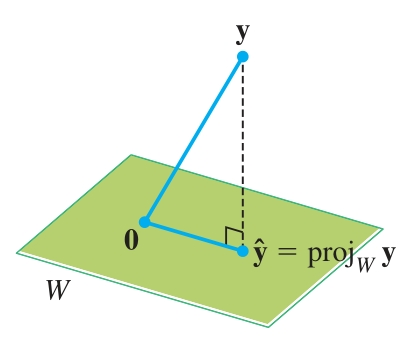
\includegraphics[width=0.25\textwidth]{images/projection-col.jpg}
    \caption{$\Hat{\B{y}}$ is the projection of $\mathbf{y}$ onto $W$, where $W$ is the column space of $\B{X}$.}
   %\label{Find the principal axes.}
    \end{figure}
\begin{Rem}
    In linear model, we are interested in the difference of the response vector $\mathbf{y}$ and its projection onto the column space of design matrix $X$. The \textbf{Sum of Squares due error} is a measurement for that purpose, which is defined as:
    \begin{equation} \label{SSE}
        \text{SSE}(\mathbf{y}) = \lVert \mathbf{y} - X\hat{\pmb{\beta}} \rVert^2 = \sum_{i = 1}^{n} (y_i - \mathbf{x}_i^{\top}\hat{\pmb{\beta}})^2
    \end{equation}
\end{Rem}

\subsection{Orthogonal Projection Matrix}
    By \cref{y-estimator}, we can see that the effect of 
    $X(X^{\top}X)^{-1}X^{\top}$ is to project $\B{y}$ onto $\text{Col}(X)$, which is why it is called \textbf{(Orthogonal) Projection Matrix}. The projection matrix is also called \textbf{Hat Matrix} in statistics. The hat matrix differs from \cref{inner product}, which projects a vector onto a vector, \textbf{while the hat matrix projects a vector onto the column space of $X$}.

\begin{Rem}
    The hat matrix is typically denoted by $H$, it has the following properties:
    \begin{enumerate}
        \item $H$ is symmetric and thus a square matrix.
        \item $H^2 = H$.
        \item If $\mathbf{x}\in\text{Col}(X)$, $H\mathbf{x} = \mathbf{x}$.
    \end{enumerate}
\end{Rem}

\begin{Def}
    \textbf{Idempotent Matrix:} A square matrix $A$ is said to be idempotent if and only if $A^2 = A$.
\end{Def}

\begin{Def}
    \textbf{Orthogonal Projection Matrix}: A matrix $P$ is an orthogonal projection matrix if $P$ is \textbf{idempotent and symmetric}.
    \begin{Rem}
    For any vector $\B{y}$, $P$ projects $\B{y}$ onto a subspace $W$, resulting in $\Hat{\B{y}} = P\B{y}$. If we project $\Hat{\B{y}}$ onto $W$ again, the equation
    \begin{equation}
        \Hat{\B{y}} = P\Hat{\B{y}} = PP\B{y} = P^2\B{y}
    \end{equation} illustrated why $P$ is needed to be \textbf{\textcolor{cyan}{idempotent}}. Conversely, suppose we want to project a vector $\B{y}$ onto a subspace $W$ spanned by $\mathcal{B} = \{\B{v}_1, \B{v}_2,\cdots, \B{v}_n \}$, we can find an orthonormal base by Gram-Schmidt Process, say $\mathcal{U} = \{\B{u}_1, \B{u}_2, \cdots, \B{u}_n\}$. By \cref{orthonormal-projection}, 
    \begin{equation*}
        \hat{\B{y}} = U\T{U}\B{y}
    \end{equation*}
    If we let $P = U\T{U}$, $P$ is clearly \textbf{\textcolor{cyan}{symmetric}}. Note also that \textbf{\textcolor{orange}{$P$ projects a vector onto the subspace spanned by the columns (or rows, since $P$ is symmetric) of $P$}}.
    \end{Rem}
\end{Def}
    We have already known that the hat matrix $H$ is the orthogonal projection matrix onto the column space of $X$, and the residual vector
    \begin{equation*}
        \hat{\epsv} = (\B{y} - H\B{y}) = (I - H)\B{y}
    \end{equation*}
    is orthogonal to $\text{Col}(X)$. It is intuitive to say that $I - H$ is the orthogonal projection matrix onto $\text{Col}(X)^\perp$ or $\text{Nul}(\T{X})$. 
    \begin{Thm}
        If $P$ is an orthogonal projection matrix, then $I - P$ is an orthogonal projection matrix onto $\text{Col}(P)^\perp$ (or $\text{Row}(P)^\perp$, since $P$ is symmetric.
    \end{Thm}
    \begin{Thm}\label{0-1-eigen}
        The eigenvalues of an orthogonal projection matrix $P$  are either $1$'s or $0$'s.
        \begin{proof}
            Since $\forall\mathbf{x}\in\text{Col}(P)$: $H\mathbf{x} = \mathbf{x}$, $\text{Col}(P)$ is an eigenspace of $P$ corresponding to the eigenvalue $1$. And $\forall \B{v}\in \text{Col}(P)^\perp: P\B{v} = 0\cdot \B{v}$ says that $\text{Col}(P)^\perp$ is another eigenspace of $P$ corresponding to eigenvalue $0$. $P$ is a $n\times n$ symmetric matrix, and $\text{dim}\Big(\text{Col}(P)\Big) + \text{dim}\Big(\text{Col}(P)^\perp\Big) = n$, so by \cref{spectral-theorem} $H$ can only have eigenvalues of $0$ or $1$.
        \end{proof}
    \end{Thm}
    \begin{Thm}
        An orthogonal projection matrix is semi-positive definite.
        \begin{proof}
            By \cref{0-1-eigen} and \cref{11-2}.
         \end{proof}
    \end{Thm}

    \begin{Ex}
        Let a quadratic form $Q(\B{x}) = \T{\B{x}}(I - H_0)\B{x}$, where $H_0$ is the projection matrix onto $\mathbbold{1}$ as discussed in \cref{H-0}. Given a vector, what does $Q(\B{x})$ stand for?
        \begin{align*}
            Q(\B{x}) &= \T{\B{x}}(I - H_0)\B{x}\\
            & = \norm{\B{x}}^2 - \T{\B{x}}H_0 \B{x}\\
            & = \norm{\B{x}}^2 - \T{\B{x}}\bar{x}\mathbbold{1}\\
            & = \norm{\B{x}}^2 - \bar{x}\sum_{i = 1}^n x_i\\
            & = \norm{\B{x}}^2 - n\bar{x}^2\\
            & = \sum_{i = 1}^n (x_i - \bar{x})^2 = (n - 1) S^2
        \end{align*}
        where $S^2$ is the sample variance.
    \end{Ex}
\subsection{Application in Linear Model}

    We have calculated $SST$ by \cref{SST}, and we want to calculate the projection vector of $\mathbf{y} - H_0\mathbf{y}$ onto $\text{Col}(X)$
    \begin{equation*}
        H(\mathbf{y} - H_0\mathbf{y}) = H\mathbf{y} - HH_0\mathbf{y} = X\hat{\pmb{\beta}} - \overline{\mathbf{y}}\ \mathbbold{1}
    \end{equation*}
    where $H\mathbf{y}$ is the prediction vector by \cref{y-estimator} and $HH_0\mathbf{y} = H_0\mathbf{y}$ since $H_0\mathbf{y}$ is in $\text{Col}(X)$.
    That is so-called \textbf{Sum of Squares due to Regression}, which is defined as:
    \begin{equation} \label{SSR}
        \text{SSR}(\mathbf{y}) = \lVert X\hat{\pmb{\beta}} - \overline{y}\ \mathbbold{1} \rVert^2 = \sum_{i = 1}^n (\mathbf{x}_i^{\top}\hat{\pmb{\beta}} - \overline{y})^2
    \end{equation}
\begin{Thm}
    We have calculated $SST$, $SSR$ and $SSE$, there is a relationship between them:
    \begin{equation}
        \text{SST}(\mathbf{y}) = \text{SSR}(\mathbf{y}) + \text{SSE}(\mathbf{y})
    \end{equation}
    Or equivalently,
    \begin{equation}\label{7-10}
        \lVert \mathbf{y} - \overline{y}\ \mathbbold{1} \rVert^2 = \lVert X\hat{\pmb{\beta}} - \overline{y}\ \mathbbold{1} \rVert^2 + \lVert \mathbf{y} - X\hat{\pmb{\beta}} \rVert^2
    \end{equation}

    \begin{proof}
        It can be proved by Pythagorean Theorem as shown in \cref{SST-SSE-SSR}.
    \end{proof}
\end{Thm}
\begin{figure}
    \centering
    \begin{tikzpicture}[x=0.75pt,y=0.75pt,yscale=-1,xscale=1]
%uncomment if require: \path (0,300); %set diagram left start at 0, and has height of 300

%Shape: Parallelogram [id:dp8573879965454236] 
\draw   (200.5,117) -- (437.33,117) -- (335.83,213) -- (99,213) -- cycle ;
%Straight Lines [id:da6339390874989326] 
\draw    (200.5,117) -- (274.3,89.71) ;
\draw [shift={(277.11,88.67)}, rotate = 159.7] [fill={rgb, 255:red, 0; green, 0; blue, 0 }  ][line width=0.08]  [draw opacity=0] (8.93,-4.29) -- (0,0) -- (8.93,4.29) -- cycle    ;
%Straight Lines [id:da41453773904723956] 
\draw [color={rgb, 255:red, 189; green, 16; blue, 224 }  ,draw opacity=1 ][fill={rgb, 255:red, 80; green, 227; blue, 194 }  ,fill opacity=1 ]   (274.83,90.61) -- (254.86,107.58) -- (231.42,127.51) -- (217.11,139.67) ;
\draw [shift={(277.11,88.67)}, rotate = 139.64] [fill={rgb, 255:red, 189; green, 16; blue, 224 }  ,fill opacity=1 ][line width=0.08]  [draw opacity=0] (8.93,-4.29) -- (0,0) -- (8.93,4.29) -- cycle    ;
%Straight Lines [id:da9150196516290705] 
\draw    (200.5,117) -- (247.46,188.16) ;
\draw [shift={(249.11,190.67)}, rotate = 236.58] [fill={rgb, 255:red, 0; green, 0; blue, 0 }  ][line width=0.08]  [draw opacity=0] (8.93,-4.29) -- (0,0) -- (8.93,4.29) -- cycle    ;
%Straight Lines [id:da9030848701120191] 
\draw [color={rgb, 255:red, 208; green, 2; blue, 27 }  ,draw opacity=1 ]   (277.04,91.67) -- (275.11,170) ;
\draw [shift={(277.11,88.67)}, rotate = 91.41] [fill={rgb, 255:red, 208; green, 2; blue, 27 }  ,fill opacity=1 ][line width=0.08]  [draw opacity=0] (8.93,-4.29) -- (0,0) -- (8.93,4.29) -- cycle    ;
%Straight Lines [id:da21384699037270427] 
\draw [color={rgb, 255:red, 126; green, 211; blue, 33 }  ,draw opacity=1 ]   (217.11,139.67) -- (272.45,168.61) ;
\draw [shift={(275.11,170)}, rotate = 207.61] [fill={rgb, 255:red, 126; green, 211; blue, 33 }  ,fill opacity=1 ][line width=0.08]  [draw opacity=0] (8.93,-4.29) -- (0,0) -- (8.93,4.29) -- cycle    ;
%Shape: Arc [id:dp9998963237475307] 
\draw  [draw opacity=0] (231.42,127.51) .. controls (233.07,130.45) and (234.25,133.72) .. (234.85,137.24) .. controls (235.51,141.08) and (235.41,144.87) .. (234.66,148.46) -- (205.58,142.23) -- cycle ; \draw  [color={rgb, 255:red, 74; green, 144; blue, 226 }  ,draw opacity=1 ] (231.42,127.51) .. controls (233.07,130.45) and (234.25,133.72) .. (234.85,137.24) .. controls (235.51,141.08) and (235.41,144.87) .. (234.66,148.46) ;  

% Text Node
\draw (284,76.4) node [anchor=north west][inner sep=0.75pt]  [font=\footnotesize]  {$\mathbf{Y}$};
% Text Node
\draw (200,149.4) node [anchor=north west][inner sep=0.75pt]    {$\mathbbold{1}$};
% Text Node
\draw (282,129.4) node [anchor=north west][inner sep=0.75pt]  [font=\footnotesize,color={rgb, 255:red, 208; green, 2; blue, 27 }  ,opacity=1 ]  {$\norm{\B{Y} - \Hbeta}^2$};
% Text Node
\draw (236.18,136.95) node [anchor=north west][inner sep=0.75pt]  [font=\scriptsize,color={rgb, 255:red, 189; green, 16; blue, 224 }  ,opacity=1 ,rotate=-317.37]  {$\norm{\B{Y} - \Bar{Y}\mathbbold{1}}^2$};
% Text Node
\draw (258.12,177.03) node [anchor=north west][inner sep=0.75pt]  [font=\footnotesize,color={rgb, 255:red, 184; green, 233; blue, 134 }  ,opacity=1 ,rotate=-0.69]  {$\norm{\widehat{\B{Y}} - \Bar{Y}\mathbbold{1}}^2$};
% Text Node
\draw (150,177.4) node [anchor=north west][inner sep=0.75pt]    {$\text{Col}(\B{X})$};
% Text Node
\draw (224,133.4) node [anchor=north west][inner sep=0.75pt]  [font=\scriptsize]  {$\theta $};
\end{tikzpicture}
    \caption{SST, SSE and SSR form a right triangle.}
    \label{SST-SSE-SSR}
\end{figure}
\begin{Thm}\label{7-3}
    Suppose $V$ is subspace of $\mathbb{R}^p$, and $W$ is a subspace of $V$, that is, $W\subseteq V$ and $\text{dim}(W) \leq \text{dim}(V)$. Then
    \begin{equation}
        \forall \mathbf{y}\in\mathbb{R}^p: \lVert \text{proj}_{V}(\mathbf{y})  \rVert \geq \lVert \text{proj}_{W}(\mathbf{y})  \rVert
    \end{equation}
    \begin{proof}

        By \cref{7-1}, $\mathbf{y} = \text{proj}_{W}(\mathbf{y}) + \mathbf{r}_W = \text{proj}_{V}(\mathbf{y}) + \mathbf{r}_V$.
        Since $W\subseteq V$, $\text{proj}_{V}(\mathbf{y}) - \text{proj}_{W}(\mathbf{y}) \in V$. We can draw a triangle with $\mathbf{r}_W$ as the hypotenuse, $\mathbf{r}_V$ and $\text{proj}_{V}(\mathbf{y}) - \text{proj}_{W}(\mathbf{y})$ as the legs. we have
        \begin{equation}\label{r-inequality}
            \lVert \mathbf{r}_W \rVert > \lVert \mathbf{r}_V \rVert + 
            \lVert \text{proj}_{V}(\mathbf{y}) - \text{proj}_{W}(\mathbf{y}) \rVert
        \end{equation}
        It indicates that $\lVert \mathbf{r}_W \rVert > \lVert \mathbf{r}_V \rVert$. By Pythagorean Theorem
        \begin{equation*}
            \lVert \mathbf{y}\rVert^2 = \lVert \text{proj}_{W}(\mathbf{y})\rVert ^2 + \lVert \mathbf{r}_W \rVert ^2 = \lVert \text{proj}_{V}(\mathbf{y})\rVert ^2 + \lVert \mathbf{r}_V \rVert ^2
        \end{equation*}
        Thus, $\lVert \text{proj}_{V}(\mathbf{y})  \rVert > \lVert \text{proj}_{W}(\mathbf{y})  \rVert$. Note that $\lVert \text{proj}_{V}(\mathbf{y})  \rVert = \lVert \text{proj}_{W}(\mathbf{y})  \rVert$ if and only if $V = W$.
    \end{proof}
\end{Thm}
The \cref{7-3} provides \textbf{\textcolor{cyan}{an interesting insight for the design matrix $X$. If we add a new column (or a new feature) into $X$, resulting in a new matrix $\Tilde{X}$, then $\text{SSE}(\mathbf{y})$ would not increase.}} Looking at \cref{7-10}, $\lVert \mathbf{y} - \overline{y}\ \mathbbold{1} \rVert^2$ is a constant and $\lVert \mathbf{r}_V\rVert = \lVert \mathbf{y} - \Tilde{X}\hat{\pmb{\beta}}\rVert \leq \lVert \mathbf{y} - X\hat{\pmb{\beta}}\rVert = \lVert \mathbf{r}_W\rVert$ as in \cref{r-inequality}, since $\text{dim}(X) \leq \text{dim}(\Tilde{X})$. Therefore, \textbf{\textcolor{magenta}{in no case will the $SSE$ increase, because the model now has more capacity to minimize the residuals (or in other words, it has more freedom to find a better fit).}}
\par
The three vectors, $\mathbf{y} - \bar{y} - \mathbbold{1}$, $X\hat{\pmb{\beta}} - \bar{y}\ \mathbbold{1}$ and $\mathbf{y} - X\hat{\pmb{\beta}}$, forms a right triangle. We can use the cosine value, as shown in \cref{SST-SSE-SSR}, to reflect the length of $\mathbf{y} - X\hat{\pmb{\beta}}$:
\begin{equation*}
    \cos^2\theta = \cfrac{\text{SSR}(\mathbf{y})}{\text{SST}(\mathbf{y})}
\end{equation*}
We can see that the range of $\cos^2 \theta$ is $[0, 1]$, and its value is proportional to $\text{SSR}(\mathbf{y})$.
\begin{Def}
    \textbf{The coefficient of determination}:
    \begin{equation}
        R^2 = 1 - \cfrac{\text{SSE}(\mathbf{y})}{\text{SST}(\mathbf{y})} = \cfrac{\text{SSR}(\mathbf{y})}{\text{SST}(\mathbf{y})}
    \end{equation}
    \textbf{\textcolor{orange}{The higher the $R^2$ is, the more accurate the predictions of our model are.}}
    $R^2$ \textbf{\textcolor{red}{non-decreases (by \cref{7-3})}} as we add new features (or columns) into the design matrix $X$.
\end{Def}
\section{Data Projection}
Consider the following matrix multiplication
\begin{equation*}
    Z = XV
\end{equation*}
where $X$ = $(\mathbf{x}_1\ \cdots\ \mathbf{x}_n)^{\top}$ is $n \times p$ and $V$ is $p \times p$.
\begin{equation}
    Z = XV =\begin{bmatrix}
        \mathbf{x}_1^{\top} V\\
        \vdots\\
        \mathbf{x}_n^{\top} V\\
    \end{bmatrix}  = 
    \begin{bmatrix}
        \mathbf{z}^{(1)}\\
        \vdots\\
        \mathbf{z}^{(n)}
    \end{bmatrix}
\end{equation}
$\mathbf{z}^{(i)} = \mathbf{x}_{i}^{\top} V$ can be considered as a linear combination of rows of $V$ using the entries in $\mathbf{x}_i^{\top}$ as weights. This implies
\begin{equation*}
    \mathbf{x}_i = V^{\top}(\mathbf{z}^{(i)})^{\top}
\end{equation*}
$(\mathbf{z}^{(i)})^{\top}$ is the coordinate of $\mathbf{x}_i$ relative to the rows of $V$. Furthermore, the $j^{\text{th}}$ entry, $z_{ij} =  \mathbf{x}_i^{\top} \mathbf{v}_j$, in $(\mathbf{z}^{(i)})^{\top}$ is the scalar projection of $\mathbf{x}_i^{\top}$ on $\mathbf{v}_j$ or on $\text{span}(\mathbf{v}_j)$. Looking at (11), let $X_j = X\mathbf{v}_j \otimes \mathbf{v}_j$ and $\mathbf{x}_j^{(i)}$ be the $i^{\text{th}}$ row of $X_j$, then
\begin{equation*}
    \mathbf{x}_j^{(i)} = \mathbf{x}_i^\top\mathbf{v}_j\mathbf{v}_j^{\top} = z_{ij}\mathbf{v}_j^{\top}
\end{equation*}
which is the projection vector of $\mathbf{x}_i^{\top}$ on $\mathbf{v}_j$.
That is, \textbf{the rows of $X_j$ are the vector projections of rows of $X$ on $\mathbf{v}_j^{\top}$}.

\noindent Since all the rows of $X_j$ are the projections on $\mathbf{v}_{j}^{\top}$, we have
\begin{equation*}
    \text{rank}(\mathbf{v}_j \otimes \mathbf{v}_j) =1 \Longrightarrow \text{rank}(X_j) = 1
\end{equation*}
All data points (or rows) of $X_j$ are on the line that goes through the origin and vector $\mathbf{v}_j^{\top}$. It says that we can restore $XV$ to $X$ by right-multiplying it by $V^{\top}$
\begin{align*}
        XVV^{\top} &=  X \mathbf{v}_1 \otimes \mathbf{v}_1 + \cdots + X \mathbf{v}_n \otimes \mathbf{v}_n\\
        & = X_1 + \cdots + X_n\\
        & = X
\end{align*}
Again, each row of $XV$ represents the coordinate of $(\mathbf{v}_1\ \cdots \ \mathbf{v}_p)^{\top}$. By right-multiplying it by its inverse $V^\top$, we can restore the coordinates to those of \textbf{standard orthonormal basis}. Another way to view $XVV^{\top}$ is as the sum of 
the projections of all data points onto the orthonormal basis. 


\section{Rank and Trace}
\subsection{Rank}
\begin{Def}
    The \textbf{rank} of a matrix $A\in \mathbb{R}^{n\times p}$ is the number of its linearly independent columns (or rows), which is expressed as $\text{rank}(A)$.
\end{Def}
\noindent 
Given a matrix $A\in \mathbb{R}^{n\times p}$, it has the following properties:
\begin{enumerate}
    \item $\text{rank}(A) = \min\{n, p \}$
    \item $\text{rank}(AB) = \min\{\text{rank}(A), \text{rank}(B) \}$
    \item Given two non-singular matrices $B\in\mathbb{R}^{n\times n}$ and $C\in\mathbb{R}^{p\times p}$:
    \begin{equation}
        \text{rank}(BA) = \text{rank}(AC) = \text{rank}(A)
    \end{equation}
    \item $\text{rank}(A^\top A) = \text{rank}(AA^{\top}) = \text{rank}(A) = \text{rank}(A^{\top})$
\end{enumerate}
Note that: property 4 illustrates that \textbf{multiplying A by a non-singular matrix does not change the rank of $A$}.

\begin{Ex}
    Show that if a matrix $A\in\mathbb{R}^{n\times p}$ with $n\geq p$ is of full column rank, then $A^{\top}A$ is non-singular.
\end{Ex}
\begin{proof}
    Since $A$ is of full column rank and $n\geq p$, we have
    \begin{equation*}
        \text{rank}(A) = p = \text{rank}(A^\top A)
    \end{equation*}
    Since $A^\top A$ is a $p\times p$ matrix and has full column rank, it is non-singular.
\end{proof}

\begin{Ex}
    Show that if a matrix $A\in\mathbb{R}^{n\times p}$ with $n\geq p$ is not of full column rank, then $A^{\top}A$ is singular.
\begin{proof}
    Since $A$ is not of full column rank, 
    \begin{equation*}
        \text{rank}(A) = \text{rank}(A^{\top} A) < p
    \end{equation*}
    It implies that $A$ is singular.
\end{proof}
\end{Ex}

\begin{Ex}
    Show that given a matrix $A\in\mathbb{R}^{n\times p}$ with $n < p$, $A^{\top}A$ is singular.
    \begin{proof}
        Since $\text{rank}(A) \leq \min\{n, p \}$,
        \begin{equation*}
            \text{rank}(A) = \text{rank}(A^{\top} A) \leq n < p
        \end{equation*}
        Since $A^\top A$ is not of full column rank, it is singular.
    \end{proof}
\end{Ex}

\subsection{Trace}
\begin{Def}
    The trace of a square matrix $A\in \R^{n \times n}$ is the sum of diagonal elements of $A$. It is denoted $\tr(A) = \sum_{i = 1}^n = a_{ii}$.
\end{Def}

\begin{Thm}\label{trace}
    The trace function $\tr(\cdot)$ has the following properties:
    \begin{enumerate}
        \item $\tr(cA \pm dB) = c\tr(A) \pm d\tr(B)$, where $c, d\in \R$.
        \item Given two matrices $A\in\R^{n\times p}, B\in \R^{p\times n}$, then $\tr(AB) = \tr(BA)$
        \begin{proof}
            Let $t_i$ be the $i^{\text{th}}$ elements on the diagonal of $AB$. Then
            \begin{equation*}
                \tr(AB) = \sum_{i = 1}^n t_i = \sum_{i = 1}^n\sum_{j = 1}^p a_{ij}b_{ji} = \sum_{j = 1}^p \sum_{i = 1}^n b_{ji}a_{ij} = \tr(BA)
            \end{equation*}
            Note that $n$ is not required to be greater or equal to $p$.
        \end{proof}

    \item Given an $n\times p$ matrix, $A = \begin{bmatrix}
        \B{a}_1 & \B{a}_2 & \cdots & \B{a}_p
    \end{bmatrix}$, $\tr(\T{A}A) = \displaystyle \sum_{i = 1}^p \T{\B{a}}_i \B{a}_i$
    \item Given an $n \times p$ matrix, $\tr(A\T{A}) = \displaystyle \sum_{i = 1}^ n \B{a}^{(i)} \B{a}_i$, where $\B{a}^{(1)}$ is the row vector of $A$.
    \item By property 3 and 4, $\tr(\T{A}A) = \tr(A\T{A}) = \displaystyle \sum_{i = 1}^n\sum_{j = 1}^p a_{ij}^2$
    \item $\tr(\E(\B{X})) = \E(\tr(\B{X}))$, where $\E$ represents the expectation of a random matrix.
    \end{enumerate}
\end{Thm}
\section{Eigenvalues and Diagonalization}
\subsection{Eigenvectors}
\begin{Def}
    Given a square matrix $A\in\mathbb{R}^{n\times n}$, there exists a vector $\mathbf{x}\in \Rn \setminus \{\mathbf{0}\}$ such that
    \begin{equation} \label{eigen}
        \exists \lambda \in \mathbb{R}:\ A\mathbf{x} = \lambda\mathbf{x}
    \end{equation}
    where $\lambda$ is called an \textbf{eigenvalue} of $A$; $\mathbf{x}$ is called an \textbf{eigenvector corresponding to $\lambda$}.
\end{Def}

\noindent 
    The \cref{eigen} can be rewritten as
    \begin{equation} \label{eigen-1}
        (A - \lambda I)\mathbf{x} = \mathbf{0}
    \end{equation}
This implies that \textbf{the set of all solutions of \cref{eigen-1}} is just the null space $\text{Nul}(A - \lambda I)$. So this set is a \textit{subspace} of $\mathbb{R}^n$ and its called the \textbf{eigenspace} of $A$ corresponding to $\lambda$.

\begin{Def}
    A scalar $\lambda$ is an eigenvalue of a matrix $A\in\mathbb{R}^n$ if and only if $\lambda$ satisfies the \textbf{characteristic equation}:
    \begin{equation}\
        \text{det}(A - \lambda I) = 0
    \end{equation}
\end{Def}

\begin{Rem}
    $A\mathbf{x} = 0\mathbf{x}$ holds if and only if $A$ is singular. That is, \textbf{$0$ is an eigenvalue of $A$ in and only if $A$ is singular}.
\end{Rem}

\begin{Thm}
    The eigenvalues of a \textbf{triangular matrix} are the entries on its main diagonal.
\end{Thm}

\begin{Thm}
    If $\mathbf{v}_1, \cdots, \mathbf{v}_r$ are eigenvalues that correspond to distinct eigenvalues $\lambda_1, \lambda_2, \cdots, \lambda_r$, then the set $\{\mathbf{v}_1, \cdots, \mathbf{v}_r \}$ is 
    \textbf{linearly independent}.
\end{Thm}

\subsection{Similarity}
\begin{Def}\label{10-3}
    If $A$ and $B$ are $n\times n$ matrices, then $A$ is similar to $B$ if there is a non-singular matrix $P$ such that
    \begin{equation*}
        P^{-1}AP = B
    \end{equation*}
\end{Def}

\begin{Thm}
    Given two matrices $A, B\in\mathbb{R}^{n\times n}$, if $A$ and $B$ are similar, then they have the same characteristic polynomial and hence the same eigenvalues(with the same multiplicities).
    \begin{Rem}
        However, $A$ and $B$ having the exactly same eigenvalues does not imply that $A$ and $B$ are similar.
    \end{Rem}
\end{Thm}

\subsection{Diagonalization}
In many cases, the eigenvalue-eigenvector information contained within a matrix $A$ can be displayed in a useful factorization for the form $A = PDP^{-1}$ where $D$ is a diagonal matrix. 
\begin{Thm}
    \textbf{The Diagonalization Theorem}: Given a matrix $A\in\mathbb{R}^{n\times n}$, $A$ is diagonalizable if and only if $A$ has $n$ linearly independent eigenvectors.
    \begin{Rem}
        In fact $A = PDP^{-1}$, if and only if the columns of $P$ are $n$ \textbf{linearly independent} eigenvectors of $A$. In this case, the diagonal entries of $D$ are eigenvalues of $A$ that correspond, resprectively, to the eigenvectors in $P$.
    \end{Rem}
\end{Thm}
\noindent In other words, $A$ is diagonalizable if and only if there are enough eigenvectors to form a basis of $\mathbb{R}^n$, which is called an \textbf{eigenvector basis} of $\mathbb{R}^n$.

\begin{Thm}
    An $n\times n$ mateix with $n$ \textbf{distinct eigenvalues} is diagonalizable.
\end{Thm}

\begin{Thm}
    Let $A$ be an $n\times n$ matrix whose distinct eigenvalues are $\lambda_1, \cdots, \lambda_p$.
    Let $\text{dim}(\mathcal{E}(\lambda_k))$ denote the dimension of eigenspace for  $\lambda_k$. The matrix $A$ is diagonalizable if and only if
    \begin{equation*}
        \sum_{i = 1} ^{p} \text{dim}(\mathcal{E}(\lambda_i)) = n
    \end{equation*}
\end{Thm}

\begin{Thm}
    If $A$ with $p$ distinct eigenvalues is diagonalizable and $\mathcal{B}_k$ is a basis for the eigenspace corresponding to $\lambda_k$, then the total collection of vectors in the sets $\mathcal{B}_1, \cdots, \mathcal{B}_p$ forms an eigenvector basis in $\mathbb{R}^n$.
\end{Thm}

\subsection{Eigenvectors and Linear Transformation}
We have already understood the simple linear transformation $A\mathbf{x}$. The goal of this section is to understand the nested transformation of $A = PDP^{-1}$.
\begin{Def}
    \textbf{Standard Matrix}:
    Any Linear transformation $T: \mathbb{R}^p \mapsto \mathbb{R}^n$ can be implemented via left-multiplication by a matrix $A$, called the \textbf{standard matrix} of $T$.
\end{Def}

\noindent Let $V$ be a $p$-dimensional vector space, let $W$ be an $n$-dimensional vector space, and let $T$ be any linear transformation from $V$ to $W$. To associate a matrix with $T$, choose ordered bases $\mathcal{B}$ and $\mathcal{C}$ for $V$ and $W$, respectively.  
\indent $\forall \mathbf{x}\in V$, the coordinate vector $[\mathbf{x}]_{\mathcal{B}}$ is in $\mathbb{R}^p$, and the coordinate vector of its image, $[T(\mathbf{x})]_{\mathcal{C}}$ is in $\mathbb{R}^n$.
    if $\mathbf{x} = r_1\mathbf{b}_1 + r_1\mathbf{b}_2 + \cdots + r_1\mathbf{b}_p$, then 
    \begin{equation*}
        [\mathbf{x}]_{\mathcal{B}} = \begin{bmatrix}
            r_1 \\
            \vdots \\
            r_p
        \end{bmatrix}
    \end{equation*} and 
    \begin{equation}\label{10-4-1}
        T(\mathbf{x}) = T( r_1\mathbf{b}_1 + r_1\mathbf{b}_2 + \cdots + r_1\mathbf{b}_p) = r_1T(\mathbf{b}_1) + r_2T(\mathbf{b}_2) + \cdots + r_pT(\mathbf{b}_p)
    \end{equation}
    Since the coordinate mapping from $W$ to $\mathbb{R}^n$ is linear, \cref{10-4-1} leads to
    \begin{equation}\label{10-4-2}
        [T(\mathbf{x})]_{\mathcal{C}} = r_1[T(\mathbf{b}_1)]_{\mathcal{C}} + r_2[T(\mathbf{b}_2)]_{\mathcal{C}} + \cdots + r_p[T(\mathbf{b}_p)]_{\mathcal{C}}
    \end{equation}
    Since $\mathcal{C}$-coordinate vecotrs are in $\mathbb{R}^n$, the vector \cref{10-4-2} can be written as a matrix equation, namely,
    
    \begin{equation}\label{10-4-3}
        [T(\mathbf{x})]_{\mathcal{C}} = M[\mathbf{x}]_{\mathcal{B}}
    \end{equation}     
    where
    \begin{equation*}
        M = \begin{bmatrix}
            T(\mathbf{b}_1)]_{\mathcal{C}} & T(\mathbf{b}_2)]_{\mathcal{C}} & \cdots & T(\mathbf{b}_p)]_{\mathcal{C}}
        \end{bmatrix}
    \end{equation*}
    The matrix $M$ is a matrix representation of $T$, called the \textbf{matrix for $T$ relative to the bases $\mathcal{B}$ and $\mathcal{C}$}.
    In the common case where $W$ is the same as $V$ and the basis $\mathcal{C}$ is the same as $\mathcal{B}$, the matrix $M$ in \cref{10-4-3} is called the \textbf{matrix for $T$ relative to $\mathcal{B}$}, or simply the \textbf{$\mathcal{B}$-matrix for $T$}, and is denoted by $[T]_{\mathcal{B}}$.
        The $\mathcal{B}$-matrix for $T: V\to V$ satisfies:
        \begin{equation*}
            [T(\mathbf{x})]_{\mathcal{B}} = [T]_{\mathcal{B}}[\mathbf{x}]_{\mathcal{B}}
        \end{equation*}
    \begin{Thm}
        \textbf{Diagonal Matrix Representation}:
        Suppose $A = PDP^{-1}$, where $D$ is a diagonal $n\times n$ matrix. If $\mathcal{B}$ is the basis for $\mathbb{R}^n$ formed from the columns of $P$, then $D$ is the $\mathcal{B}$-matrix for the transformation.

        \begin{proof} \label{10-8}
            Let $\mathcal{B} = \{\mathbf{b}_1, \cdots, \mathbf{b}_n\}$ and $P = \begin{bmatrix}
                \mathbf{b}_1 & \cdots & \mathbf{b}_n
            \end{bmatrix}$. In this case, $P$ is the change-of-coordinates matrix $P_{\mathcal{B}}$ discussed in \cref{4-1}, where
            \begin{equation*}
                P[\mathbf{x}]_{\mathcal{B}} = \mathbf{x}\quad \text{and}\quad [\mathbf{x}]_{\mathcal{B}} = P^{-1}\mathbf{x}
            \end{equation*}
            If $T(\mathbf{x}) = A\mathbf{x}$ for $\mathbf{x} \in \mathbb{R}^n$, then
            \begin{align*}
                [T]_{\mathcal{B}} &= \begin{bmatrix}
                    [T(\mathbf{b}_1)]_{\mathcal{B}} & \cdots & [T(\mathbf{b}_n)]_{\mathcal{B}}
                \end{bmatrix}\\
                & = \begin{bmatrix}
                    [A\mathbf{b}_1]_{\mathcal{B}} & \cdots & [A\mathbf{b}_n]_{\mathcal{B}}
                \end{bmatrix}\\
                & = \begin{bmatrix}
                    P^{-1}A\mathbf{b}_1 & \cdots & P^{-1}A\mathbf{b}_n
                \end{bmatrix}\\
                & = P^{-1}A \begin{bmatrix}
                    \mathbf{b}_1 & \cdots & \mathbf{b}_n
                \end{bmatrix}\\
                & = P^{-1}AP = D
            \end{align*}
                 
        \end{proof}
    \end{Thm}

    \begin{Rem}
        The proof of \cref{10-8} didn't use the information that $D$ was diagonal. Hence, if $A$ is similar to a matrix $C$, with $A = PCP^{-1}$, then $C$ is the $\mathcal{B}$-matrix for the transformation $\mathbf{x}\mapsto A\mathbf{x}$ when the basis $\mathcal{B}$ is formed from the columns of $P$. Multiplying by such a matrix $A$  has the following interpretation: given a vector $\mathbf{x}\in V$
        \begin{enumerate}
            \item $P^{-1}\mathbf{x} \mapsto [\mathbf{x}]_{\mathcal{B}}$
            \item $C[\mathbf{x}]_{\mathcal{B}} \mapsto [A\mathbf{x}]_{\mathcal{B}}$
            \item $P[A\mathbf{x}]_{\mathcal{B}}\mapsto A\mathbf{x}$
        \end{enumerate}
        
        
        \begin{center}
            \begin{tikzpicture}
              \matrix (m) [matrix of math nodes,row sep=3em,column sep=4em,minimum width=2em]
              {
                 \B{x} & A\B{x} \\
                 \left[\B{x} \right]_{\mathcal{B}} & \left[A\B{x} \right]_{\mathcal{B}} \\
                };
                
              \path[-stealth]
                (m-1-1) edge node [left] {$P^{-1}$} (m-2-1)
                        edge [left] node [below] {$A$} (m-1-2)
                (m-2-1.east|-m-2-2) edge node [below] {$C$} (m-2-2)
                (m-2-2) edge node [right] {$P$} (m-1-2);
            \end{tikzpicture}
        \end{center}

        
        
        Conversely, if $T:\mathbb{R}^n\to \mathbb{R}^n$ is defined by $T(\mathbf{x}) = A\mathbf{x}$, and if $\mathcal{B}$ is any basis for $\mathbb{R}^n$, then the $\mathcal{B}$-matrix for $T$ is similar to $A$. The \cref{10-8} show that if $P$ is the matrix whose columns come from the vectors in $\mathcal{B}$, then
        \begin{equation*}
            [T]_{\mathcal{B}} = P^{-1}AP
        \end{equation*}
        Thus, the set of all matrices similar to a matrix $A$ \textbf{coincides with the set of all matrix representations of the transformation $\mathbf{x}\mapsto A\mathbf{x}$}.
    \end{Rem}

    \subsection{Symmetric Matrices}
    \begin{Def}
        A \textbf{symmetric} matrix is a matrix $A$ such that $A^{\top} = A$. Note that such a matrix is necessarily square.

    \end{Def}
    \begin{Thm}
        If $A$ is symmetric, then any two eigenvectors from different eigenspaces are orthogonal.

        \begin{proof}
            Suppose there are two eigenvectors $\mathbf{v}_1, \mathbf{v}_2$, respectively, corresponding to distinct eigenvalues $\lambda_1$ and $\lambda_2$. Consider the following equation:
            \begin{align*}
                \lambda _1 \mathbf{v}_1^{\top}\mathbf{v}_2 & = (A\mathbf{v}_1)^{\top} \mathbf{v}_2\\
                & = \mathbf{v}_1^{\top} A^{\top}\mathbf{v}_2\\
                & = \mathbf{v}_1^{\top} A\mathbf{v}_2\quad \text{since } A \text{ is a symmetric matrix}\\
                & = \lambda _2 \mathbf{v}_1^{\top} \mathbf{v}_2
            \end{align*}
            We can get $(\lambda_1 - \lambda_2)\mathbf{v}_1^{\top} \mathbf{v}_2 = 0$. Since $\lambda_1 \neq \lambda_2$, $\mathbf{v}_1^{\top} \mathbf{v}_2$ must be $0$.
        \end{proof}
    \end{Thm}
    \begin{Def}
        \textbf{Orthogonally dianonalizable:} For an $n \times n$ matrix $A$, if there are an \textbf{orthogonal matrix} $P$ with ($P^{-1} = P^{\top}$) and a diagonal matrix $D$ such that 
        \begin{equation}\label{10-6}
            A = PDP^{\top} = PDP^{-1}
        \end{equation}
        then $A$ is said to be \textbf{Orthogonally dianonalizable}.

        \begin{Rem}
            Such a diagonalization requires $n$ \textbf{linearly independent} and \textbf{orthonormal eigenvectors}.
            If $A$ is orthogonally diagonalizable as in \cref{10-6}, then
            \begin{equation*}
                A^{\top} = (PDP^{\top})^{\top} = PDP^{\top} = A
            \end{equation*}
            Thus, $A$ is symmetric.
        \end{Rem}
    \end{Def}

    \begin{Thm}\label{orthogonally-dianonalizable}
        An $n\times n$ matrix $A$ is orthogonally diagonalizable if and only if $A$ is a symmetric matrix.
    \end{Thm}

    \begin{Thm}\label{spectral-theorem}
        \textbf{The Spectral Theorem for Symmetric Matrices}:
        An $n \times n$ matrix $A$ has the following properties:
        \begin{enumerate}
            \item $A$ has $n$ real eigenvalues, counting multiplicities.
            \item The dimension of the eigenspace for each eigenvalue $\lambda$ equals the multiplicity of $\lambda$ as a root of the characteristic equation.
            \item  The eigenspaces are mutually orthogonal, in the sense that eigenvectors corresponding to different eigenvalues are orthogonal.
            \item $A$ is orthogonally diagonalizable.
        \end{enumerate}
    \end{Thm}

    \begin{Thm}
        \textbf{Spectral Decomposition}:
        Suppose $A$ is orthogonally diagonalizable,
        \begin{align*}
            A =& PDP^{\top} = \begin{bmatrix}
                [\mathbf{u}_1 & \cdots & \mathbf{u}_n] 
            \end{bmatrix} \begin{bmatrix}
                \lambda_1 & 0 & 0 & \cdots & 0 \\
                \vdots & \vdots & \vdots & \ddots & \vdots \\
                0 & 0 & 0 & \cdots & \lambda_n
                \end{bmatrix} \begin{bmatrix}
                    \mathbf{u}_1^{\top}\\
                    \vdots\\
                    \mathbf{u}_n^{\top}
                \end{bmatrix}\\
                & = \begin{bmatrix}
                \lambda_1 \mathbf{u}_1 & \cdots & \lambda_n \mathbf{u}_n
            \end{bmatrix} \begin{bmatrix}
                    \mathbf{u}_1^{\top}\\
                    \vdots\\
                    \mathbf{u}_n^{\top}
                \end{bmatrix}
        \end{align*}
        Using the \cref{sum-outer}, the sum of outer product representation:
        \begin{equation}
            A = \lambda_1\mathbf{u}_1\mathbf{u}_1^{\top} + \lambda_2\mathbf{u}_2\mathbf{u}_2^{\top} + \cdots + \lambda_n\mathbf{u}_n\mathbf{u}_n^{\top}
        \end{equation}
        This representation of $A$ is called a \textbf{spectral decomposition} of $A$. Note each $\mathbf{u}_i\mathbf{u}_1i{\top}$ is a projection matrix with rank $1$.
    \end{Thm}
    \subsection{Intuition of Unit Eigenvectors}
    Suppose that a symmetric matrix $A\in\mathbb{R}^2$ with two \textit{unit} eigenvectors $\mathbf{v}_1$ and $\mathbf{v}_2$, which are orthogonal to each other.
    \begin{enumerate}
    \item 
     We can find a unit circle that goes through the four points: $\mathbf{v}_1, \mathbf{v}_2, -\mathbf{v}_1, -\mathbf{v}_2$. After multiplying the four vectors by $A$, we can find an ellipse that goes through these fore vectors.
    \item Suppose $A\in\mathbb{R}^{n\times n}$ can be diagonalized into 
    \begin{equation*}
        A = PDP^{-1}
    \end{equation*}
    Right-multiplying $A$ by $P$:
    \begin{equation*}
        AP =  \begin{bmatrix}
            A\mathbf{v}_1 & A\mathbf{v}_2 
        \end{bmatrix} = 
        \begin{bmatrix}
            \lambda_1\mathbf{v}_1 & \lambda_2\mathbf{v}_2
        \end{bmatrix}
    \end{equation*}
    We can find an ellipse that goes through the columns of $AP$. Actually $P$ is an orthogonal matrix, its effect is to perform \textbf{a rotational transformation}, mapping a coordinate vector relative to $\{\mathbf{v}_1, \mathbf{v}_2 \}$ to a vector in the standard basis. While the effect of the diagonal matrix $D$ is to perform \textbf{a scaling transformation}.
    \item Consider the linear transformation $T(\mathbf{x}) = A\mathbf{x}$,
    \begin{equation*}
        A\mathbf{x} = PDP^{-1}\mathbf{x} = \mathbf{y}
    \end{equation*}
    $P^{-1}\mathbf{x} = [\mathbf{x}]_{\mathcal{B}}$ maps $\mathbf{x}$ into a new coordinate system with a set of orthonormal basis as its coordinate vectors, which corresponds to a \textbf{rotational action}. $D[\mathbf{x}]_{\mathcal{B}} = [\mathbf{y}]_{\mathcal{B}}$ scales the vector. $P[\mathbf{y}]_{\mathcal{B}}$ transforms $[\mathbf{y}]_{\mathcal{B}}$ back to standard basis.  

    \item Multiplying $A$ by a vector or a matrix (a set of column vectors) corresponds to a sequence of operations: a rotation, followed by a scaling, and then a rotation back.
    \end{enumerate} 

    \subsection{Important Properties of Eigenvalues}
    If $\mathbf{v}$ is an eigenvector of $A$ corresponding to eigenvalue $\lambda$, then
    \begin{equation*}
        A^2\mathbf{v} = AA\mathbf{v} = A\lambda \mathbf{v} = \lambda ^2 \mathbf{v}
    \end{equation*}
    We can generalize the equation above to 
    \begin{equation}
        A^k\mathbf{v} = \lambda ^k \mathbf{v}
    \end{equation}
    Suppose $A\in \mathbb{R}^{n\times n}$ has $n$ eigenvalues, then
    \begin{equation}
        \text{det}(A) = \prod_{i = 1}^n \lambda_i
    \end{equation}
    \begin{proof}
        Let the characteristic equation of $A$ be
        \begin{align*}
            p(\lambda) = \text{det}(A - \lambda I) = (\lambda_1 - \lambda)\cdots (\lambda_n - \lambda)
        \end{align*}
        We can simply get the result by letting $\lambda$ be zero.
    \end{proof}

    \subsection{Spectral Decomposition on Gram Matrix}
    Given a data matrix $X\in\mathbb{R}^{n\times p}$, its Gram matrix $X^\top X$ is symmetric and, therefore, orthogonally diagonalizable by \cref{orthogonally-dianonalizable}:
    \begin{equation*}
        G = X^\top X = PDP^{\top}
    \end{equation*}
    We can get the following equation:
    \begin{equation*}
        P^{\top} GP = \begin{bmatrix}
            \mathbf{u}_1^\top X^{\top} X\mathbf{u}_1 & \mathbf{u}_1^\top X^{\top} X\mathbf{u}_2 & \cdots & \mathbf{u}_1^\top X^{\top} X\mathbf{u}_p\\
            \cdots & \cdots & \ddots & \cdots\\
            \mathbf{u}_p^\top X^{\top} X\mathbf{u}_1 & \mathbf{u}_p^\top X^{\top} X\mathbf{u}_2 & \cdots & \mathbf{u}_p^\top X^{\top} X\mathbf{u}_p
        \end{bmatrix} = 
        \begin{bmatrix}
        \lambda_1 & 0 & 0 & \cdots & 0 \\
        \vdots & \vdots & \vdots & \ddots & \vdots \\
        0 & 0 & 0 & \cdots & \lambda_n
        \end{bmatrix}
    \end{equation*}
    Let $X\mathbf{u}_i = \mathbf{y}_i$, the $k^{\text{th}}$ entry of $\mathbf{y}_i$ is the projection of the $k^{\text{th}}$ data point (the $k^{\text{th}}$ row of $X$) onto the eigenvector $\mathbf{u}_i$.
    \begin{equation*}
        P^{\top}GP = \begin{bmatrix}
            \mathbf{y}_1^\top \mathbf{y}_1 & \mathbf{y}_1^\top \mathbf{y}_2 & \cdots & \mathbf{y}_1^\top \mathbf{y}_p\\
            \cdots & \cdots & \ddots & \cdots\\
            \mathbf{y}_p^\top \mathbf{y}_1 & \mathbf{y}_p^\top \mathbf{y}_2& \cdots & \mathbf{y}_p^\top \mathbf{y}_p
        \end{bmatrix} = D
    \end{equation*}
    For any $i \neq j$, we can see that $\mathbf{y}_i$ and $\mathbf{y}_j$ are orthogonal to each other. Meanwhile, $\lVert \mathbf{y_i} \rVert^2 = \lambda_i$, which means
    \begin{equation*}
        \sum_{j = 1}^{p} y_{ij}^2 = \lambda_i
    \end{equation*}
    That is, the sum of squares of the coordinates of each data point relative to $\mathbf{y}_i$ equals to $\lambda_i$. This means that the projections of data points (rows) of $X$ onto different eigenvectors of $G$ have different sums of squares. We can express $G$ in its spectral decomposition form:
    \begin{equation}
        G = \lambda_1\mathbf{u}_1\mathbf{u}_1^{\top} + \lambda_2\mathbf{u}_2\mathbf{u}_2^{\top} + \cdots + \lambda_n\mathbf{u}_n\mathbf{u}_n^{\top}
    \end{equation}
    The equation above indicates that \textbf{\textcolor{cyan}{the larger the eigenvalue, the more important the eigenvector}}, as the projections of data points onto it are larger.

    \subsection{Change of Variable}
    Suppose $A\in\Rnn$ has $n$ eigenvectors $\{\B{v}_1, \B{v}_2, \cdots, \B{v}_n \}$, which can form a basis $\mathcal{B}$ for $\Rn$. Let $\begin{bmatrix}
        \B{v}_1 & \cdots & \B{v}_n
    \end{bmatrix}$. Given a sequence $\{\B{x}_k\}$ satisfying 
    \begin{equation*}
        \B{x}_{k + 1} = A\B{x}_k
    \end{equation*} which is called a difference equation. Define a new sequence $\{\B{y}_{k}\}$ by
    \begin{equation*}
        \B{y}_{k} = P^{-1}\B{x}_k,\quad \text{or equivalently,}\quad \B{x}_k = P\B{y}_k    \end{equation*}
    $\B{y}_{k}$ is clearly the coordinate of $\B{x}_k$ relative to $\mathcal{B}$ by \cref{4-1}.
    Substituting these relations into the equation $\B{x}_{k + 1} = A\B{x}_k$ and using the fact that $A = PDP^{-1}$:
    \begin{equation*}
        \B{x}_{k + 1} = AP\B{y}_{k} = PDP^{-1}P\B{y}_k = PD\B{y}_{k}
    \end{equation*}
    Left-multiplying the above equation by $P^{-1}$:
    \begin{equation*}
        P^{-1}\B{x}_{k + 1} =\B{y}_{k + 1} =  D\B{y}_k
    \end{equation*}
    The change of variable from $\B{x}_k$ to $\B{y}_k$ has \textbf{decoupled} the system of difference equations. Geometrically, the only effect on $\B{y}_k$ is scaling the vector, and each entry $y_{i}$ of $\B{y}_k$ is unaffected by the other entries. \textbf{\textcolor{orange}{Decoupling the system allows for the calculation in a new coordinate system, which demonstrates the power of linear algebra.}}
\section{TODO: Quadratic Form}
    \begin{Def}\label{def-quadratic}
        A \textbf{quadratic form on $\Rn$} is a function $Q: \Rn\to \mathbb{R}$ whose input vector $\B{x}$ can be computed by an expression of the form:.
        \begin{equation*}
            Q(\B{x}) = \B{x}^{\top}A\B{x}
        \end{equation*}
        where $A$ is a $n\times n$ \textit{symmetric matrix} and called \textbf{the matrix of the quadratic form}. Since $A$ is symmetric, $Q(\B{x})$ can also be expressed as:
        \begin{equation*}
            Q(\B{x}) = \B{x}^{\top}A\B{x} = \sum_{i = 1}^n a_{ii}x_i^2 + 2\sum_{i = 1}^{n - 1}\sum_{j = i + 1}^n a_{ij}x_{i}x_{j}
        \end{equation*}
    \end{Def}
    \subsection{Change of Variable in a Quadratic Form}
    Let $\B{x}\in\Rn$, then a \textit{change of variable} is an equation of the form
    \begin{equation*}
        \B{x} = P\B{y},\quad \text{or equivalently} \quad \B{y} = P^{-1}\B{x}
    \end{equation*}
    where $P$ is a non-singular $n\times n$ matrix. It is easy to see $\B{y} = \coo{x}{B}$, where $\mathcal{B}$ is the set of columns of $P$. Then
    \begin{equation}
        Q(\B{x}) = \B{x}^{\top}A\B{x} = (P\mathbf{y})^{\top} A(P\B{y}) = \B{y}^{\top}(P^{\top}AP)\B{y} = \T{\B{y}}D\B{y}
    \end{equation}
    which uses the fact that $A$ is symmetric.
    \begin{Ex}
        Let
        \begin{equation*}
            A = \begin{bmatrix}
                a & c\\
                c & b
            \end{bmatrix}, \B{x} = \begin{bmatrix}
                x_1\\
                x_2
            \end{bmatrix}
        \end{equation*}
        where $A$ has eigenvalues $\lambda_1$ and $\lambda_2$. Then
        \begin{equation*}
            Q(\B{x}) = \T{\B{x}}A\B{x} = a^2x_1^2 + b^2x_2 + 2cx_1x_2
        \end{equation*}
        By making the change of variable:
        \begin{equation}\label{change-of-variable}
            Q(\B{x}) = Q'(\B{y}) = \T{\B{y}}D\B{y} =  \lambda_1^2y_1^2 + \lambda_2^2y_2^2
        \end{equation}
        \begin{Rem}
            If we let $Q'(\B{y}) = 1$, then $\lambda_1^2y_1^2 + \lambda_2^2y_2^2 = 1$ represents \textbf{\textcolor{red} {an ellipse centred at the origin}}.
        \end{Rem}
    \end{Ex}
    \begin{Thm}
        \textbf{The Principal Axes Theorem}:
        Let $A\in\Rnn$ be a symmetric matrix. Then there is an orthogonal change of variable, $\B{x} = P\B{y}$, that transforms the quadratic form $\quadratic{x}{A}$ into a quadratic form $\quadratic{y}{D}$ with no cross-product term. The columns of $P$ are called the \textbf{principal axes} and $\B{y}$ is the coordinate of $\B{x}$ relative to the columns of $P$.
    \end{Thm}
    \subsection{A Geometric View of Principal Axes}
    Suppose $Q(\B{x}) = \quadratic{x}{A} = k$, where $A$ is $2\times 2$ symmetric matrix and $k\in\mathbb{R}$.
    The set of all $\B{x}\in\mathbb{R}^2$ that satisfy
    \begin{equation*}
        \quadratic{x}{A} = \quadratic{x}{A} = k
    \end{equation*}
    It can be expressed as
    \begin{equation*}
        a^2x_1^2 + bx_1x_2 + c^2x_2^2 + dx_1 + ex_2 + f = 0
    \end{equation*}
    which either corresponds to 
    \begin{enumerate}
        \item an ellipse (or a circle):
        \begin{equation}\label{ellipse}
            a^2x_1^2 + bx_1x_2 + c^2x_2^2 + dx_1 + ex_2 + f = 0,\ ac> 0
        \end{equation}
        \item a hyperbola:
        \begin{equation}\label{hyperbola}
            a^2x_1^2 + bx_1x_2 + c^2x_2^2 + dx_1 + ex_2 + f = 0,\ ac < 0
        \end{equation}
        \item two intersecting lines, if the \cref{ellipse} can be factorized to
        \begin{equation*}
            (\alpha_1x_1 + \beta_1x_2 + \gamma_1)(\alpha_2x_1 + \beta_2x_2 + \gamma_2) = 0
        \end{equation*}
        \item a single point:
        \begin{equation*}
            (x_1 - x_0)(x_2 - y_0) = 0
        \end{equation*}
    \end{enumerate}
    If $A$ is a diagonal matrix, the graph is in \textit{standard position}, which implies that the ellipse or the hyperbola is centred at the origin. Therefore, the \cref{ellipse} can be written as:
    \begin{equation*}
        \cfrac{x_1}{a^2} + \cfrac{x_2}{b^2} = 1,\ a>0,\ b > 0
    \end{equation*}
    The \cref{hyperbola} can be written as:
    \begin{equation*}
        \cfrac{x_1}{a^2} - \cfrac{x_2}{b^2} = 1,\ a>0,\ b > 0
    \end{equation*}
    \textbf{\textcolor{cyan}{Find the \textit{principal axes} (determined by the eigenvectors of $A$) amounts to finding a new coordinate system with respect to which the graph is in standard position (centred at the origin)}}, as shown below:
    \begin{figure}[ht]
    \centering
    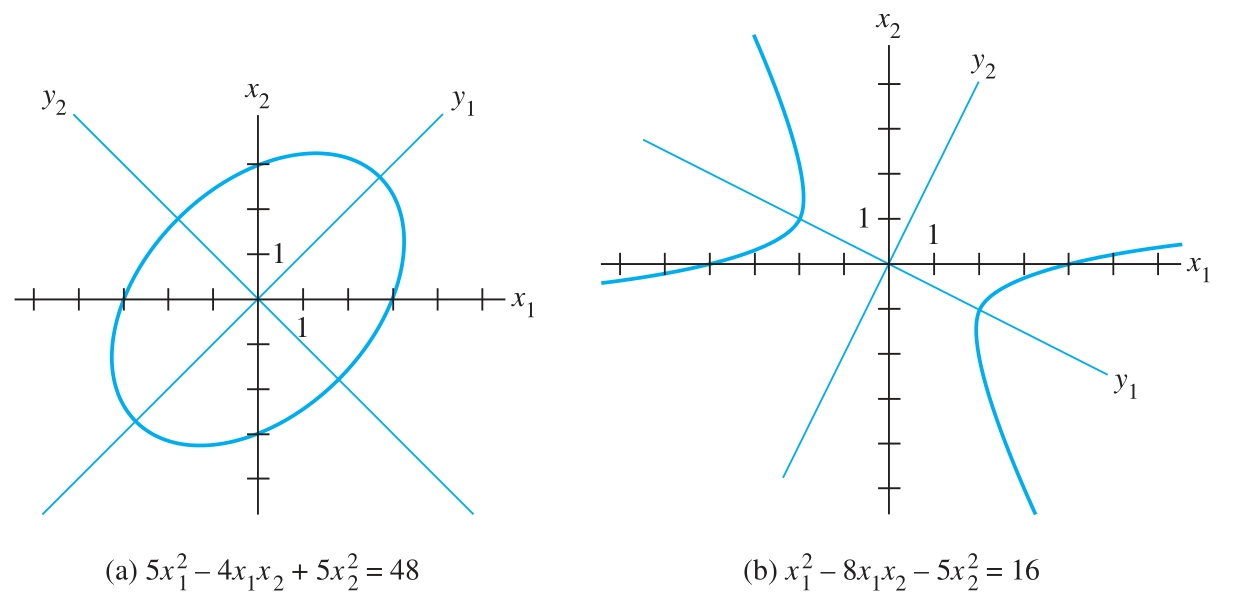
\includegraphics[width=0.75\textwidth]{images/principal-axes.png}
    \caption{Finding the principal axes.}
   %\label{Find the principal axes.}
    \end{figure}
    
    \subsection{Classifying Quadratic Forms}
    \begin{Def}\label{quad-def}
        A quadratic from $Q$ is
        \begin{enumerate}[(a)]
            \item \textbf{positive definite} if $\forall \B{x} \neq \B{0}:Q(\B{x}) > 0$
             \item \textbf{negative definite} if $\forall \B{x} \neq \B{0}:Q(\B{x}) < 0$
             \item \textbf{indefinite} if $Q(\B{x})$ assumes both positive and negative values.
             \item \textbf{positive semi-definite} if $\forall \B{x}:Q(\B{x}) > 0$
             \item \textbf{negative semi-definite} if $\forall \B{x}:Q(\B{x}) < 0$
        \end{enumerate}

    \end{Def}
        As shown in the figure 2.
        \begin{figure}
        \centering
        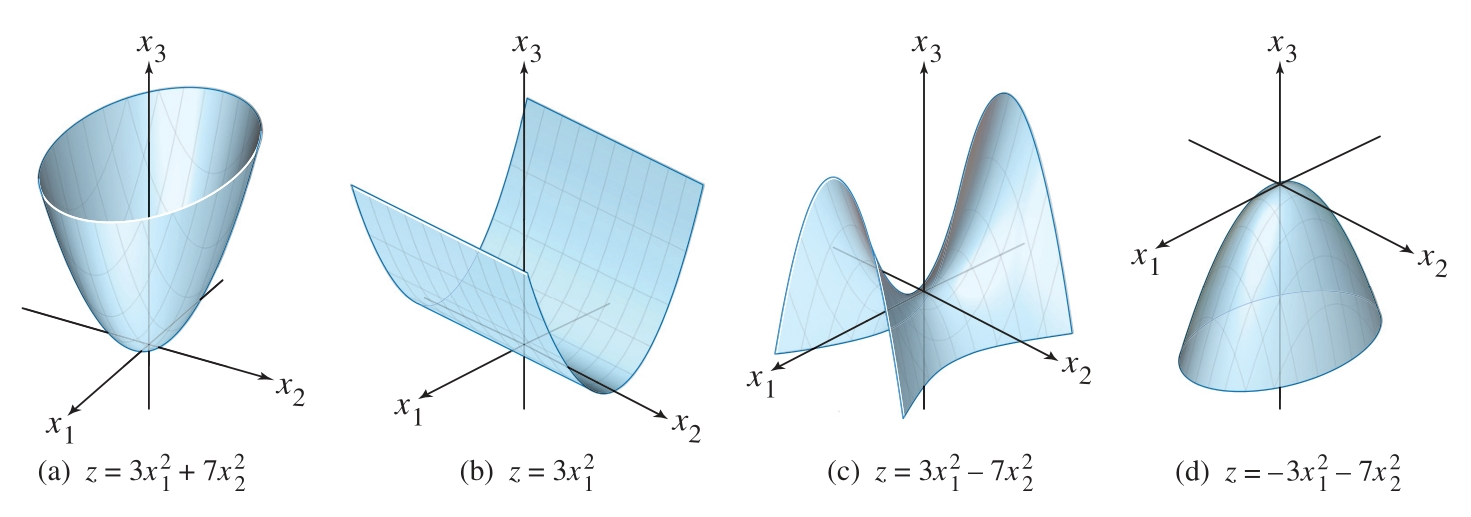
\includegraphics[width=0.75\textwidth]{images/quadratic-class.png}
        \caption{Graphs of quadratic forms.}
       %\label{Find the principal axes.}
        \end{figure}
        
    \begin{Thm}\label{11-2}
        \textbf{Quadratic Forms and Eigenvalues}:
        Given a quadratic form $Q(\B{x}) = \quadratic{x}{A}$, then $Q$ is
        \begin{enumerate}[a.]
            \item positive definite if and only if the eigenvalues of $A$ are all positive,
            \item negative definite if and only if the eigenvalues of $A$ are all negative, or
            \item indefinite if and only $A$ has both positive and negative eigenvalues.
        \end{enumerate}
        \begin{proof}
            By the \cref{change-of-variable},
            \begin{equation}
                Q(\B{x}) = \quadratic{x}{A} = \quadratic{y}{D} = \sum_{i = 1}^n  \lambda_iy_i^2
            \end{equation}
            Since $P$ is non-singular, there is a one-to-one relation between $\B{x}$ and $\B{y}$. For any nonzero $\B{x}$, the right side of the equation above coincides with $Q(\B{x})$ for $\B{x}\neq \B{0}$. Thereore, $Q(\B{x})$ is obviously controlled by the signs of the eigenvalues of $A$, in the three ways described in the theorem.
        \end{proof}
        \begin{Rem}
            If $A$ has a nonzero eigenvalue, say $\lambda_k = 0$, then $A\B{x} = 0$ has a non-trivial solution, implying $\exists\B{x}\neq \B{0}: Q(\mathbf{x}) = 0$.
        \end{Rem}
    \end{Thm}
\section{TODO: A preview of Constrained Optimization}
    \subsection{Subject to a Unit Vector}
    In some applications, we often need to find the maximum or minimum value of a quadratic form $Q(\B{x)}$ for $\B{x}$ in some specified set. For example,
    \begin{equation*}
        c = \underset{\lVert \B{x} \rVert = 1}{\argmin}\ Q({\B{x}})
    \end{equation*}
    
    \begin{figure}[ht]
    \centering
    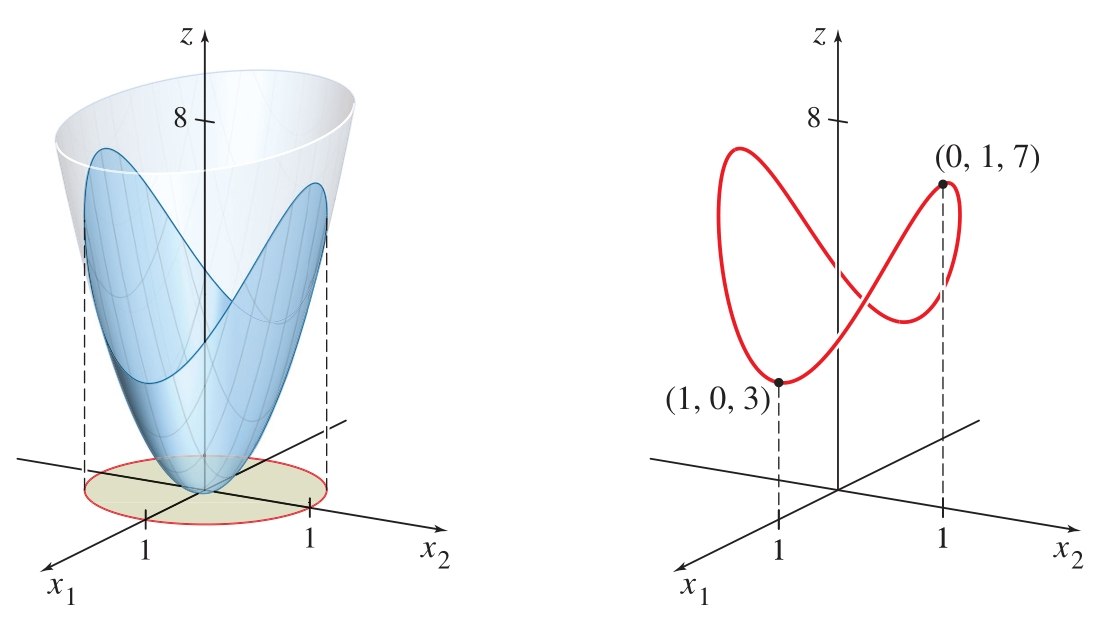
\includegraphics[width=0.6\textwidth]{images/constrained-1.jpg}
    \caption{$z = 3x_1^2 + 7x_2^2$ constrained on $x_1^2+x_2^2 = 1$}
   %\label{Find the principal axes.}
    \end{figure}

    \begin{Thm}\label{unit-opt}
        Given a quadratic form $Q(\B{x})$, and let $m = \underset{\lVert \B{x} \rVert = 1}{\argmin}\ Q({\B{x}})$ and $M = \underset{\lVert \B{x} \rVert = 1}{\argmax}\ Q({\B{x}})$. then 
        \begin{enumerate}
            \item $M$ is the greatest eigenvalue $\lambda_1$ of $A$
            \item $m$ is the least eigenvalue $\lambda_n$ of $A$.
        \end{enumerate}
        The value of $\quadratic{x}{A}$ is
        \begin{enumerate}
            \item $M$ when $\B{x}$ is a unit eigenvector $\B{u}_1$ corresponding to $\lambda_1$
            \item $m$ when $\B{x}$ is a unit eigenvector $\B{u}_m$ corresponding to $\lambda_n$
        \end{enumerate}
        \begin{proof}
            By the \cref{orthogonally-dianonalizable}, $A$ can be orthogonally diagonalized as $PDP^{-1}$, where either $P$ or $P^{-1}$ is an orthogonal matrix, thus preserving the length $\B{x}$. By \cref{change-of-variable}
            \begin{equation*}
                Q(\B{x}) = Q'(\B{y}) = \sum_{i = 1}^n \lambda_i y_i^2
            \end{equation*}
            where $\lambda$'s are arranged in descending order. The following inequality holds:
            \begin{align*}
                Q'(\B{y})\leq \lambda_1 \sum_{i = 1}^n y_i^2 = \lambda_1 \T{\B{y}}\B{y}
            \end{align*}
            where $\lambda_1$ is the largest eigenvalue of $A$. Let $\B{y}$ be $\B{e}_1$, a vector with the first entry being $1$ and the other being $0$. Then,
            \begin{equation*}
                \lambda_1 \T{\B{y}}\B{y} = \T{\B{e}_1} D\B{e}_1 
            \end{equation*}
            illustrates that $Q'(\B{y})$ reaches its maximum value when $\B{y} = \B{e}_1$, implying that $Q(\B{x})$ attains its maximum value when $\B{x} = P\B{e}_1 = \B{u}_1$. A similar method can be applied to prove its minimum value.
        \end{proof}
    \end{Thm}
    \begin{Thm}
        Given a quadratic form $Q(\B{x}) = \quadratic{x}{A}$, let $\lambda_1$ be the largest eigenvalue of $A$, and $\B{u}_1$ be the eigenvector corresponding to $\lambda_1$. then the maximum value of $Q$ subject to the following constrains:
        \begin{equation*}
            \T{\B{x}}\B{x} = 1,\quad \T{\B{x}}\B{u}_1 = 0
        \end{equation*} is the second greatest eigenvalue $\lambda_2$, and this maximum is attained when $\B{x}$ is an eigenvector $\B{u}_2$ corresponding to $\lambda_2$.
        \begin{Rem}
            Suppose that $A$ is orthogonally diagonalized as $PDP^{-1}$ with its eigenvalues arranged, in descending order, on the main diagonal of $D$. 
            If there are more constrains on $Q$:
            \begin{equation*}
                \T{\B{x}}\B{x} = 1,\quad \T{\B{x}}\B{u}_1 = 0,\quad \cdots, \T{\B{x}}\B{u}_{k - 1} = 0
            \end{equation*}
            then the maximum of $Q$ is attained at $\B{x} = \B{u}_k$ where $\B{u}_k$ is the eigenvector corresponding to the $k^{\text{th}}$ greatest eigenvalue.
        \end{Rem}
    \end{Thm}
    \section{TODO: Singular Value Decomposition}
    Unfortunately, as we know, not all matrices can be factored as $A = PDP^{-1}$ with $D$ diagonal. However, a factorization $A = QDP^{-1}$ is possible for \textit{any} $m\times n$ matrix $A$! A special factorization of this type, called the \textbf{singular value decomposition}, is \textbf{\textcolor{red}{the most useful matrix decomposition in the universe.}}\emoji{wink} \par
    If $A\B{x} = \lambda \B{x}$ and $\norm{\B{x}} = 1$, then
    \begin{equation*}
        \norm{A\B{x}} = \norm{\lambda \B{x}} = |\lambda| \norm{\B{x}} = |\lambda|
    \end{equation*} If $\lambda_1$ is the eigenvalue with the greatest magnitude, then a corresponding unit eigenvector $\B{v}_1$ identifies a direction in which the stretching effect of $A$ is greatest.

    \begin{Ex}
      If the linear transformation $\B{x}\to A\B{x}$ maps the unit sphere $\{ \B{x}: \norm{\B{x}} = 1 \}$ in $\R^3$ onto an ellipse in $\R^2$. Find a unit vector $\B{x}$ at which the length $\norm{A\B{x}}$ is maximized, and compute this maximum length.
      \begin{sol}
          The quantity $\norm{A\B{x}}^2$ is maximized at the same $\B{x}$ that maximizes $\norm{A\B{x}}$, 
          \begin{equation*}
              \norm{A\B{x}}^2 = \T{(A\B{x})}(A\B{x}) = \T{\B{x}}(\T{A}A)\B{x}
          \end{equation*} Since $\T{A}A$ is symmetric, so the problem is reduced into maximizing the quadratic form $\T{\B{x}}(\T{A}A)\B{x}$ subject to the constraint $\norm{\B{x}} = 1$ as discussed in \cref{unit-opt}. Hence, the maximum value is the greatest eigenvalue $\lambda_1$ of $\T{A}A$, and the maximum value is attained at a unit eigenvector of $\T{A}A$ corresponding to $\lambda_1$.
      \end{sol}
    \end{Ex}
    The example above suggests that the effect of $A$ on the unit sphere in $\R^3$ is related to the quadratic form $\T{x}(\T{A}A)\B{x}$.\par 
    Let $A\in\R^{m\times n}$. Then $\T{A}A$ can be orthogonally diagonalized. Let $\{\B{v}_1, \cdots, \B{v}_n \}$ be an orthonormal basis for $\R^n$ consisting of eigenvectors of $\T{A}A$. Then,
    \begin{equation}\label{t}
        \norm{A\B{v}_i} = \T{(A\B{v}_i)}A\B{v}_i = \T{\B{v}_i}(\lambda_i \B{v}_i) = \lambda_i\geq 0
    \end{equation}Note that $\norm{\B{v}_i} = 1$. So \textbf{\textcolor{orange}{the eigenvalues of $\T{A}A$ are all non-negative, implying that $\T{A}A$ is a semi-positive definite matrix.}}
    \begin{Def}
        The singular values of $A$ are the square roots of the eigenvalues of $\T{A}A$, denoted by $\sigma_1, \cdots, \sigma_n$, and they are arranged in decreasing order. By \cref{t}, the \textbf{singular values of $A$ are the lengths of the vectors $A\B{v}_1, \cdots, A\B{v}_n$}. 
        \begin{Rem}
            The first two singular values of $A$ are the lengths of the major and minor semi-axes of the ellipse as shown \cref{singular-ellipse}.
        \end{Rem}
    \end{Def}
    \begin{figure}
        \centering
        \begin{tikzpicture}[x=0.75pt,y=0.75pt,yscale=-1,xscale=1]
%uncomment if require: \path (0,300); %set diagram left start at 0, and has height of 300

%Shape: Axis 2D [id:dp5842664307886825] 
\draw  (216,137) -- (454.11,137)(335.11,49) -- (335.11,241) (447.11,132) -- (454.11,137) -- (447.11,142) (330.11,56) -- (335.11,49) -- (340.11,56)  ;
%Shape: Ellipse [id:dp9660000625734635] 
\draw  [color={rgb, 255:red, 74; green, 144; blue, 226 }  ,draw opacity=1 ][line width=1.5]  (280.59,181.88) .. controls (266.65,164.95) and (279.76,131.13) .. (309.87,106.34) .. controls (339.99,81.55) and (375.7,75.18) .. (389.64,92.12) .. controls (403.58,109.05) and (390.46,142.87) .. (360.35,167.66) .. controls (330.24,192.45) and (294.52,198.82) .. (280.59,181.88) -- cycle ;
%Straight Lines [id:da36332977734700256] 
\draw [color={rgb, 255:red, 245; green, 166; blue, 35 }  ,draw opacity=1 ][line width=1.5]    (335.11,137) -- (387.32,94.02) ;
\draw [shift={(389.64,92.12)}, rotate = 140.54] [color={rgb, 255:red, 245; green, 166; blue, 35 }  ,draw opacity=1 ][line width=1.5]    (14.21,-4.28) .. controls (9.04,-1.82) and (4.3,-0.39) .. (0,0) .. controls (4.3,0.39) and (9.04,1.82) .. (14.21,4.28)   ;
%Straight Lines [id:da7831499075107744] 
\draw [color={rgb, 255:red, 126; green, 211; blue, 33 }  ,draw opacity=1 ][line width=1.5]    (335.11,137) -- (311.78,108.65) ;
\draw [shift={(309.87,106.34)}, rotate = 50.54] [color={rgb, 255:red, 126; green, 211; blue, 33 }  ,draw opacity=1 ][line width=1.5]    (14.21,-4.28) .. controls (9.04,-1.82) and (4.3,-0.39) .. (0,0) .. controls (4.3,0.39) and (9.04,1.82) .. (14.21,4.28)   ;

% Text Node
\draw (397,76.4) node [anchor=north west][inner sep=0.75pt]    {$A\mathbf{v}_{1}$};
% Text Node
\draw (289,79.4) node [anchor=north west][inner sep=0.75pt]    {$A\mathbf{v}_{2}$};


\end{tikzpicture}
        \caption{$A\B{v}_1$ is the major semi-axis and $A\B{v}_2$ is the minor semi-axis of the ellipse.}
        \label{singular-ellipse}
    \end{figure}

    \begin{Thm}\label{t-1}
        Suppose $\{\B{v}_1, \cdots, \B{v}_n\}$ is an orthonormal basis of $\Rn$ consisting of eigenvectors of $\T{A}A$, arranged so that the corresponding eigenvalues of $\T{A}A$ satisfy $\lambda_1\geq \cdots\geq \lambda_n$, and suppose that $A$ has $r$ nonzero singular values. Then $\{A\B{v}_1, \cdots, A\B{v}_r \}$ is an orthogonal basis for $\text{Col}(A)$, and $\text{rank}(A) = r$.
        \begin{proof}
            Given two vectors $A\B{v}_j, A\B{v}_i$ where $i\neq j$, 
            \begin{equation*}
                \T{(A\B{v}_j)}A\B{v}_i = \T{\B{v}_j}\T{A}A\B{v}_i = \lambda_i \T{\B{v}_j}\B{v}_i = 0 
            \end{equation*} Thus, $\{A\B{v}_1, \cdots, A\B{v}_n \}$ is an orthogonal set. Furthermore, since the lengths of the vector $\{A\B{v}_1, \cdots, A\B{v}_n$ are the singular values of $A$, and since there are $r$ non-zero singular values, $A\B{v}_i\neq \B{0}$ if and only if $1\leq i\leq r$. So, $\{A\B{v}_1, \cdots, A\B{v}_r$ are linearly independent vectors, and they are in $\text{Col}(A)$. $\forall \B{y}\in\text{Col}(A)$, say $\B{y} = A\B{x}$ , we can write
            \begin{equation*}
                \B{x} = c_1\B{v}_1 + \cdots + c_n\B{v}_n
            \end{equation*}, and 
            \begin{align*}
                \B{y} &= A\B{x}\\
                & = c_1A\B{v}_1 + \cdots + c_rA\B{v}_r + c_{r+1}A\B{v}_{r+1} + \cdots + c_nA\B{v}_n\\
                & = c_1A\B{v}_1 + \cdots + c_rA\B{v}_r + 0 + 0 + \cdots + 0
            \end{align*} Thus $\B{y}$ is in $\text{Span}\{A\B{v}_1, \cdots, A\B{v}_r \}$, which shows that $\{ A\B{v}_1, \cdots, A\B{v}_r \}$ is an (orthogonal) basis for $\text{Col}(A)$. Hence $\text{rank}(A) = \text{dim}\Big(\text{Col}(A)\Big) = r$.
        \end{proof}
    \end{Thm}
The decomposition of $A$ involves an $m\times n$ \enquote{diagonal} matrix $\Lambda$ of the form
\begin{equation}\label{Lambda}
    \Lambda = \begin{bmatrix}
        D & \B{O}\\
        \B{O} & \B{O}
    \end{bmatrix}
\end{equation} where $D$ is an $r\times r$ diagonal matrix for some $r$ not exceeding the smaller of $m$ and $n$.

\begin{Thm}
    \textbf{The Singular Value Decomposition or (SVD)}: 
    Let $A$ be an $m\times n$ matrix with rank $r$. then there exists an $m\times n$ matrix $\Lambda$ as in \cref{Lambda} for which the diagonal entries in $D$ are the first singular values of $A$, $\sigma_1\geq \sigma_2\geq \cdots \geq \sigma_r\geq 0$, and there exist an $m\times n$ orthogonal matrix $U$ and an $n\times n$ orthogonal matrix $V$ such that
    \begin{equation*}
        A = U\Lambda \T{V}
    \end{equation*}
    \begin{proof}
        Let $\lambda_i$ and $\B{v}_i$ be as in \cref{t-1}, so that $\{A\B{v}_1, \cdots, A\B{v}_r \}$ is an orthogonal basis for $\text{Col}(A)$. Normalize each $A\B{v}_i$ to obtain an orthonormal basis $\mathcal{U} = \{\B{u}_1, \cdots, \B{u}_r \}$, where
        \begin{equation}
            \B{u}_i = \cfrac{A\B{v}_i}{\norm{A\B{v}_i}} = \cfrac{A\B{v}_i}{\sigma_i}
        \end{equation} and 
        \begin{equation}
            A\B{v}_i = \sigma_i \B{u}_i
        \end{equation} Now extend $\mathcal{U}$ to an orthonormal basis $\{ 
\B{u}_1, \cdots, \B{u}_m \}$ of $\R^m$, and let 
        \begin{equation}
            U = \begin{bmatrix}
                \B{u_1} & \cdots & \B{u}_m
            \end{bmatrix} \quad \text{and }\quad \begin{bmatrix}
                    \B{v}_1 & \cdots & \B{v}_n
                \end{bmatrix}
        \end{equation} By construction, $U$ and $V$ are orthogonal matrices. Also,
        \begin{equation}
            AV = \begin{bmatrix}
                A\B{v}_1 & \cdots & A\B{v}_r & \B{0} & \cdots & \B{0} 
            \end{bmatrix} = \begin{bmatrix}
                    \sigma_1\B{u}_1 & \cdots & \sigma_r\B{u}_r & \B{0} & \cdots & \B{0}
                \end{bmatrix}
        \end{equation} Let $D$ be the diagonal matrix with diagonal entries $\sigma_1,\cdots, \sigma_r$, and let $\Lambda$ be as in \cref{t-1} above. Then
        \begin{equation}
            U\Lambda = \begin{bmatrix}
                U_1 & U_2
            \end{bmatrix} \begin{bmatrix}
                    D & \B{O}\\
                    \B{O} & \B{O}
                \end{bmatrix} = \begin{bmatrix}
                    U_1 D & \B{O}
                \end{bmatrix} = AV
        \end{equation}
        where $U_1 = \begin{bmatrix}
            \B{u}_1 & \cdots & \B{u}_r
        \end{bmatrix}$ and $U_2 = \begin{bmatrix}
            \B{u}_{r+1} & \cdots & \B{u}_{m}
        \end{bmatrix}$. Since $V$ is an orthogonal matrix,
        \begin{equation*}
            U\Lambda \T{V} = AV\T{V} = A
        \end{equation*}
    \end{proof}
    \begin{Rem}
            The columns of $U$ are called \textbf{left singular vectors} of $A$, and the columns of $V$ are called \textbf{right singular vectors} of $A$.
    \end{Rem}
\end{Thm}
\subsection{Bases for Fundamental Subspaces}
Given an SVD decomposition for a $m\times n$ matrix $A$, by observing its left singular vectors, we can find that $\{\B{u}_1, \cdots, \B{u}_r \}$ is an orthonormal basis for $\text{Col}(A)$ by \cref{t-1}, and $\{\B{u}_{r+1}, \cdots, \B{u}_n\}$ is an orthonormal basis for $\text{Nul}(\T{A})$, since for any $r< i\leq n$, $\B{u}_i$ is orthogonal to $\text{Col}(A) = \text{Span}\{\B{u}_1, \cdots, \B{u}_{r} \}$, that is, $\text{Span}\{\B{u}_{r+1}, \cdots, \B{u}_m \} = \text{Col}(A)^\perp$.\par
    Since $\{\B{u}_1, \cdots, \B{u}_r \}$ forms a basis for $\text{Col}(A)$, $\text{dim}(A) = r$, implying $\text{dim}\Big(\text{Nul}(A) \Big) = n - r$. For any $i > r$, since $A\B{v}_i = \B{0}$ and $\text{dim}\Big(\text{Nul}(A) \Big) = n - r$, $\text{Span}\{\B{v}_{r+1}, \cdots, \B{v}_{n} \} = \text{Nul}(A)$. Note that $\text{Nul}(A)^\perp = \text{Row}(A)$. Hence, $\{\B{v}_1,\cdots, v_r \}$ is an orthonormal basis for $\text{Row}(A)$. Observing that
    \begin{equation*}
        AV = \begin{bmatrix}
                A\B{v}_1 & \cdots & A\B{v}_r & \B{0} & \cdots & \B{0} 
            \end{bmatrix} = \begin{bmatrix}
                    \sigma_1\B{u}_1 & \cdots & \sigma_r\B{u}_r & \B{0} & \cdots & \B{0}
                \end{bmatrix}
    \end{equation*} for which the non-zero vectors of $AV$ is an orthogonal basis for $\text{Col}(A)$. In other words, the matrix $A$ transforms a collection of basis vectors of $\text{Col}(A)$ and $\text{Nul}(\T{A})$ into a collection of basis of $\text{Row}(A)$ and $\text{Nul}(A)$. 
    
    Let $V = \begin{bmatrix}
        \B{v}_1 & \cdots & \B{v}_r
    \end{bmatrix}$, $\begin{bmatrix}
        \B{v}_{r+1} & \cdots & \B{v}_{n}
    \end{bmatrix}$. And let $U_1 = \begin{bmatrix}
        \B{u}_1 & \cdots & \B{u}_r
    \end{bmatrix}$, $\begin{bmatrix}
        \B{u}_{r+1} & \cdots & \B{u}_{m}
    \end{bmatrix}$, they have the relationship shown as \cref{SVD-relation},
    \begin{figure}
        \centering
        \begin{tikzpicture}[x=0.75pt,y=0.75pt,yscale=-1,xscale=1]
%uncomment if require: \path (0,300); %set diagram left start at 0, and has height of 300


% Text Node
\draw (278,88.4) node [anchor=north west][inner sep=0.75pt]    {$\text{Span}(U_{1}) =\text{Col}(A)$};
% Text Node
\draw (289,156.4) node [anchor=north west][inner sep=0.75pt]    {$\text{Span}(U_{2}) =\text{Nul}\left( A^{\top }\right)$};
% Text Node
\draw (67,102.4) node [anchor=north west][inner sep=0.75pt]    {$\text{Row}(A) =\text{Span}(V_{1})$};
% Text Node
\draw (65,156.4) node [anchor=north west][inner sep=0.75pt]    {$\text{Nul}(A)=\text{Span}(V_{2})$};
% Text Node
\draw (226,70.4) node [anchor=north west][inner sep=0.75pt]    {$A$};
% Text Node
\draw (233,135.4) node [anchor=north west][inner sep=0.75pt]    {$A$};
% Connection
\draw    (195,170.6) .. controls (210.41,191.15) and (235,136.53) .. (284.49,156.63) ;
\draw [shift={(286,157.26)}, rotate = 203.39] [color={rgb, 255:red, 0; green, 0; blue, 0 }  ][line width=0.75]    (10.93,-3.29) .. controls (6.95,-1.4) and (3.31,-0.3) .. (0,0) .. controls (3.31,0.3) and (6.95,1.4) .. (10.93,3.29)   ;
% Connection
\draw    (154.9,98) .. controls (195.13,67.3) and (229.57,104.33) .. (273.66,96.98) ;
\draw [shift={(275,96.74)}, rotate = 169.44] [color={rgb, 255:red, 0; green, 0; blue, 0 }  ][line width=0.75]    (10.93,-3.29) .. controls (6.95,-1.4) and (3.31,-0.3) .. (0,0) .. controls (3.31,0.3) and (6.95,1.4) .. (10.93,3.29)   ;

\end{tikzpicture}
        \caption{The effect of $A$ on $V$.}
        \label{SVD-relation}
    \end{figure}
\section{Vector Calculus}
    \subsection{Gradient}
    \begin{Def}
        \textbf{Gradient}: Let $f:\mathbb{R}^n\to \mathbb{R}$. The gradient of the function $f$ with respect to $\mathbf{x}$ is a vector of $n$ partial derivatives:
        \begin{equation}
            \nabla_{\mathbf{x}} f(\mathbf{x}) = \begin{bmatrix}
                \partial_{x_1}f(\mathbf{x}) & 
                \partial_{x_2}f(\mathbf{x}) & 
                \cdots &
                \partial_{x_n}f(\mathbf{x})
            \end{bmatrix}^{\top}
        \end{equation}
        $\nabla_{\mathbf{x}} f(\mathbf{x})$ is typically replaced by $\nabla f(\mathbf{x})$.
    \end{Def}
    \noindent The following rules come in handy for differentiating multivariate function:
    \begin{enumerate}
        \item  $\forall A \in\mathbb{R}^{n\times p}$: $\nabla_{\mathbf{x}} A\mathbf{x} = A^{\top}$
        \item $\forall A \in\mathbb{R}^{p\times p}$: $\nabla_{\mathbf{x}}\mathbf{x}^{\top}A \mathbf{x} = (A + A^{\top})\mathbf{x}$
        \item $\nabla_{\mathbf{x}}\lVert \mathbf{x} \rVert^2 = \nabla_{\mathbf{x}}\mathbf{x}^{\top}\mathbf{x} = 2\mathbf{x}$
    \end{enumerate}
    \begin{Thm}\label{Chain-rule}
        \textbf{Chain Rule:}
        Suppose $y = f(\mathbf{u})$ has variables $u_1, u_2, \cdots, u_m$. where each $u_i = g_i(\mathbf{x})$ has variables $x_1, x_2, \cdots, x_n$, i.e., $\mathbf{u} = g(\mathbf{x})$. Then
        \begin{equation}
            \cfrac{\partial y}{\partial x_i} = \cfrac{\partial y}{\partial u_1}\cfrac{\partial u_1}{\partial x_i} + \cfrac{\partial y}{\partial u_2}\cfrac{\partial u_2}{\partial x_i} + \cdots + \cfrac{\partial y}{\partial u_m}\cfrac{\partial u_m}{\partial x_i} = A\nabla_{\mathbf{u}} y.
        \end{equation}
        where $A \in\mathbb{R}^{n\times m}$ contains the derivative of vector $\mathbf{u}$ with respect to vector $\mathbf{x}$.
    \end{Thm}
    \begin{Ex} \label{12 - 1}
        Let $X$ be an $n\times p$ matrix, find a vector $\hat{\pmb{\beta}}$ such that
        \begin{equation*}
            \hat{\pmb{\beta}} = \underset{\mathbf{b}\in \mathbb{R}^p}{\argmin} \ \lVert \mathbf{y} - X\mathbf{b} \rVert^2
        \end{equation*}
        \begin{sol}
        Let $f(\mathbf{b}) = \lVert \mathbf{y} - X\mathbf{b} \rVert^2 = (\mathbf{y} - X\mathbf{b})^{\top}(\mathbf{y} - X\mathbf{b})$. Expanding $(\mathbf{y} - X\mathbf{b})^{\top}(\mathbf{y} - X\mathbf{b})$.
            \begin{align*}
                f(\mathbf{b}) = \mathbf{y}^{\top}\mathbf{y} - \mathbf{y}^{\top} X \mathbf{b} - \mathbf{b}^\top X^{\top}\mathbf{y} + \mathbf{b}^\top X^{\top} X\mathbf{b}
            \end{align*}
            It is easy to see the above equation has a minimum value. Let its gradient be $\mathbf{0}$:
            \begin{align*}
                \nabla f(\mathbf{b}) &= -X^{\top}\mathbf{y} - X^{\top}\mathbf{y} + 2X^{\top}X \mathbf{b} = \mathbf{0}
            \end{align*}
            If $X^{\top}X$ is non-singular, we can get $\mathbf{b} = (X^{\top}X)^{-1}X^{\top} \mathbf{y}$.
        \end{sol}
    \end{Ex}

    \subsection{Jacobin Matrix}
    Let $F:\mathbb{R}^n\to \mathbb{R}^m$ be a differentiable function on region $D\subseteq \R^m$. That is, $\forall \B{x}\in D$, 
    \begin{equation*}
        F(\B{x}) = \begin{bmatrix}
            f_1(\B{x}) & f_2(\B{x}) & \cdots & f_n(\B{x})
        \end{bmatrix}^\top
    \end{equation*}
    for which each $f_i$ is an $\R^n \to \R$ function. However, since the function $F$ can be arbitrarily complected, a good approach is to find a linear function that approximate $F$ around a point $\B{p}\in \mathbb{R}^n$. Suppose we can find such a function, say $T(\B{x}) = A\B{x} + \B{b}$. It must satisfy the following conditions:
    \begin{enumerate}
        \item $F(\B{p}) = T(\B{p})$
        \item $\displaystyle \lim_{\B{x}\to \B{p}}F(\B{p}) - T({\B{x}}) = 0 $
    \end{enumerate}
    By the first condition, $T(\B{p}) = A\B{p} + \B{b}$, we have
    \begin{equation}
        \B{b} = F(\B{p}) - A\B{p}
    \end{equation}
    Substitute equation above to $T(\B{x})$
    \begin{equation}
        T(\B{x}) = A\B{x} + F(\B{p}) - A\B{p} = F(\B{p}) + A(\B{x} - \B{p})
    \end{equation}
    Then, the condtion 2 can be written as
    \begin{equation}
        \lim_{\B{x}\to \B{p}} F(\B{x}) - F(\B{p}) + A(\B{x} - \B{p}) = 0
    \end{equation}
    We can handle a simpe case with it: let $\B{x}$ approaches to $\B{p}$ along a standard coordinate axis. Let $\B{e}_i$ be a vector, where the $i^{\text{th}}$ entry is one and all other entries are zeros, and $\B{x} = \B{p} + h\B{e}_j$. Then
    \begin{equation}
        \lim_{h\to 0} F(\B{p} + h\B{e}_j) - F(\B{p}) + A(h\B{e}_j) = 0
    \end{equation} where $h\neq 0$. The equation above is equiavalent to
    \begin{equation}
        \lim_{h\to 0} \cfrac{F(\B{p} + h\B{e}_j) - F(\B{p}) + A(h\B{e}_j)}{h} = \lim_{h\to 0} \cfrac{F(\B{p} + h\B{e}_j) - F(\B{p}) + hA(h\B{e}_j)}{h} = 0
    \end{equation}
    We can get
    \begin{equation}
        \lim_{h\to 0} \cfrac{F(\B{p} + h\B{e}_j) - F(\B{p}) }{h} = A\B{e}_j = \begin{bmatrix}
            \cfrac{\partial f_1}{\partial x_j}(\B{p}) & \cfrac{\partial f_2}{\partial x_j}(\B{p}) & \cdots & \cfrac{\partial f_m}{\partial x_j}(\B{p})
        \end{bmatrix}^{\top}
    \end{equation}
    Hence,
    \begin{equation}
        A = \begin{bmatrix}
            \cfrac{\partial f_1}{\partial x_1}(\B{p}) & \cfrac{\partial f_2}{\partial x_1}(\B{p}) & \cdots & \cfrac{\partial f_n}{\partial x_1}(\B{p})\\\\

            \cfrac{\partial f_1}{\partial x_2}(\B{p}) & \cfrac{\partial f_2}{\partial x_n}(\B{p}) & \cdots & \cfrac{\partial f_n}{\partial x_n}(\B{p})\\\\

            \vdots & \vdots & \ddots & \vdots\\\\

             \cfrac{\partial f_n}{\partial x_m}(\B{p}) & \cfrac{\partial f_n}{\partial x_m}(\B{p}) & \cdots & \cfrac{\partial f_n}{\partial x_m}(\B{p})
             \end{bmatrix}
    \end{equation}
    Note that the matrix $A$ discussed in \cref{Chain-rule} has the similar form as the above matrix.
    \begin{Def}\label{Jacobin-Matrix}
        \textbf{Jacobin Matrix}:
    Suppose $\B{y} = f(\B{x}):\Rn \to \mathbb{R}^m$ is a continuous function with continuous partial derivatives, where each $y_i = f_i(\B{x})$. Its Jacobin matrix is defined as below:
    \begin{equation}
        J_f = \nabla f(\B{x})= \begin{bmatrix}
            \cfrac{\partial f_1}{\partial x_1} & \cfrac{\partial f_2}{\partial x_1} & \cdots & \cfrac{\partial f_n}{\partial x_1}\\\\

            \cfrac{\partial f_1}{\partial x_2} & \cfrac{\partial f_2}{\partial x_n} & \cdots & \cfrac{\partial f_n}{\partial x_n}\\\\

            \vdots & \vdots & \ddots & \vdots\\\\

             \cfrac{\partial f_n}{\partial x_m} & \cfrac{\partial f_n}{\partial x_m} & \cdots & \cfrac{\partial f_n}{\partial x_m}
        \end{bmatrix}
    \end{equation}
    \end{Def}    
    \begin{Thm}
        Suppose a function $f:\Rn \to \Rn$ as discussed in \cref{Jacobin-Matrix} is invertible, then
        \begin{equation}
            \det(J_{f^{-1}}) = \det(J_f)^{-1}
        \end{equation}
    \end{Thm}


    \subsection{Multivariate Taylor's Theorem}
    We've learned Taylor series for a function $y = f(x)$ of a single variable. For an $n + 1$-times differentiable function $f : \R \to \R$, we have
    \begin{equation}
        f(x) = f(c) + f'(c)(x - c) + \cfrac{f''(c)(x - c)^2}{2!} + \cdots + \cfrac{f^{(n)}(c)(x - c)^n}{n!} + R_n(x, c)
    \end{equation}
    where $R_n(x, c)$ is called the \textbf{remained term}:
    \begin{equation}
        R_n(x ,c) = \cfrac{f^{(n+1)}(z)(x - c)^n}{n!}
    \end{equation}
    for which $z$ is a real number between $x$ and $c$.
    There is a very similar formula for functions of several variables. Before go further, let us define some notations. For a function $f:\Rn \to \R$ and  two vectors: $\B{x}_0,\B{h}\in \Rn$: 
    \begin{align*}
        D_f(\B{x}_0, \B{h}) &= \sum_{i = 1}^n \cfrac{\partial f}{\partial x_i}(\B{x}_0) h_i\\
        D^2_f(\B{x}_0, \B{h}) &= \sum_{i = 1}^n\sum_{j = 1}^n \cfrac{\partial^2 f}{\partial x_i \partial x_j}(\B{x}_0) h_ih_j\\
        D^3_f(\B{x}_0, \B{h}) &= \sum_{i = 1}^n\sum_{j = 1}^n\sum_{k = 1}^n \cfrac{\partial^3 f}{\partial x_i \partial x_j \partial x_k}(\B{x}_0) h_ih_jh_k 
    \end{align*}
    and so on. Note that $D_f(\B{x}_0, \B{h}) = \nabla f(\B{x}_0)^\top \B{h}$.
    \begin{Thm}
        Let $f:\Rn \to \R$ be an $n + 1$-times continuously differentiable function at the point $\B{v_0}\in \Rn$. Then, 
        \begin{equation*}
            f(\B{x}) = f(\B{v}_0) + \sum_{k = 1}^n \cfrac{1}{k!}D^k_{f}(\B{v}_0, \B{x} - \B{v}_0) + \cfrac{1}{(n + 1)!}D^{n + 1}_f(\B{z}, \B{x} - \B{v}_0)
        \end{equation*}
        where $\B{z}$ is some point on the segment from $\B{x}$ to $\B{v}_0$.
    \end{Thm}
    \begin{Ex}
        Write out the Taylor expansion through terms of degree $2$ for $f:\R^2 \to \R^2$. Let $\B{x} = \begin{bmatrix}
            x_1 & x_2
        \end{bmatrix}^\top$
        \begin{align*}
            f(\B{x}) &= f(\B{v}_0) + \bigg(\cfrac{\partial f}{\partial x_1}(\B{v}_0)(x_1 - v_1) + \cfrac{\partial f}{\partial x_2}(\B{v}_0)(x_2 - v_2) \bigg) + \\
            & \cfrac{1}{2}\bigg(\cfrac{\partial^2 f}{\partial x_1^2}(\B{v}_0)(x_1 - v_1)^2 + \cfrac{\partial^2 f}{\partial x_1 \partial x_2}(\B{v}_0)(x_1 - v_1)(x_2 - v_2) + \cfrac{\partial^2 f}{\partial x_2^2}(\B{v}_0)(x_2 - v_2)^2 +  \cfrac{\partial^2 f}{\partial x_2 \partial x_1}(\B{v}_0)(x_2 - v_2)(x_1 - v_1)   \bigg)\\
            & + \cdots 
        \end{align*}
        Note the term of degree $1$ can be written as $\nabla f(\B{v_0})^{\top} (\B{x} - \B{v}_0)$, and the term of degree $2$ can be written in a quadratic form:
        \begin{equation}\label{second-term}
            \cfrac{1}{2}(\B{x} - \B{v}_0)^{\top} \begin{bmatrix}
            \cfrac{\partial^2 f}{\partial x_1^2}(\B{v}_0) & \cfrac{\partial^2 f}{\partial x_2 \partial x_1}(\B{v}_0)\\\\
            \cfrac{\partial^2 f}{\partial x_1 \partial x_2}(\B{v}_0) & \cfrac{\partial^2 f}{\partial x_2^2}(\B{v}_0) 
        \end{bmatrix} (\B{x} - \B{v}_0)
        \end{equation} The matrix in \cref{second-term} is called \textbf{Hessian Matrix}, denoted by $\B{H}_f(\B{v}_0)$.
    \end{Ex}

    \subsection{TODO: Hessian Matrix}
    \begin{Def}
        Suppose $f: \Rn \to \R$ has continuous second-order derivatives. Then the Hessian Matrix is a square $n\times n$ matrix, usually defined and arranged as
        \begin{equation}
            H_f = \begin{bmatrix}
            \cfrac{\partial^2 f}{\partial x_1^2} & \cfrac{\partial^2 f}{\partial x_1 \partial x_2} & \cdots & \cfrac{\partial^2 f}{\partial x_1 \partial x_n} \\\\
            \cfrac{\partial^2 f}{\partial x_2 \partial x_1} & \cfrac{\partial^2 f}{\partial x_2^2} & \cdots & \cfrac{\partial^2 f}{\partial x_2 \partial x_n} \\\\
            \vdots & \vdots & \ddots & \vdots \\\\
            \cfrac{\partial^2 f}{\partial x_n \partial x_1} & \cfrac{\partial^2 f}{\partial x_n \partial x_2} & \cdots & \cfrac{\partial^2 f}{\partial x_n^2}
            \end{bmatrix}
        \end{equation}
    \end{Def}
    \subsection{TODO: Put them together}
\section{Probability and Statistics}
    In this section, an uppercase letter (e.g., $X$) represents a random variable, while a bold upper letter (e.g., $\mathbf{X}$) represents a random vector, random matrix, or real matrix.
    \subsection{Expectation and Variance for Random Matrix}
    \begin{Def}
        The expectation of a random vector $\X \in \Rp$ is a $p$-dimensional vector defined as:
        \begin{equation*}
            \E(\X) = \begin{bmatrix}
                \E(X_1)\\
                \E(X_2)\\
                \vdots \\
                \E(X_p)
            \end{bmatrix} = \pmb{\mu}_{\X}
        \end{equation*}
    \end{Def}

    \begin{Def}
        \textbf{Covariance Matrix:} A $p\times p$ matrix $\covmat$ defined as
        \begin{equation*}
            \covmat = \text{Var}(\X) = \E((\X - \muX{X})(\X - \muX{X})^{\top})
        \end{equation*}
        is called the covariance matrix of $\X$.
        We can expand the outer product:
        \begin{align*}
            \Var(\X) &= \begin{bmatrix}
                \E\Big((X_1 - \mu_1)^2\Big) & \E\Big((X_1 - \mu_1)(X_2 - \mu_2)\Big) & \cdots &  \E\Big((X_1 - \mu_1)(X_p - \mu_p)\Big)\\
                \vdots & \ddots  & \cdots & \vdots\\
                \E\Big((X_p - \mu_p)(X_1 - \mu_1)\Big) & \E\Big((X_p - \mu_p)(X_2 - \mu_2)\Big) & \cdots &  \E\Big((X_p - \mu_p)^2\Big)
            \end{bmatrix}\\\\
            & = \begin{bmatrix}
                \sigma_{11} & \sigma_{12} & \cdots &  \sigma_{1p}\\
                \vdots & \ddots  & \cdots & \vdots\\
                \sigma_{p1} & \sigma_{p2} & \cdots &  \sigma_{pp}
            \end{bmatrix}
        \end{align*}
        where $\sigma_{ij}$ stands for $\text{Cov}(X_i, X_j)$. It is easy to see that \textbf{$\Var(\X)$ is symmetric} due to the fact that $\text{Cov}(X_i, X_j) = \text{Cov}(X_j, X_i)$.
        \begin{Rem}
            If $\X$ and $\B{Y}$ are two random vectors with different joint probability distributions, then $\Cov(\X, \B{Y})$ is \textbf{\textcolor{red}{NOT symmetric}}, therefore $\Cov(\X, \B{Y})\neq \Cov(\B{Y}, \B{X})$.
        \end{Rem}
    \end{Def}
    \begin{Thm}
        $\Var(\X)$ has the following equivalent representation:
        \begin{equation}
            \Var(\X) = \E(\X\X^{\top}) - \muX{X}\muX{X}^{\top}
        \end{equation}
        due to the fact that $\Cov(X_i, X_j) = \E(X_iX_j) - \E(X_i)\E(X_j)$.
    \end{Thm}
    \begin{Thm}
    The following rules come in handy for calculating expectation and variance:
    \begin{enumerate}
        \item $\E(\X + \B{C}) = \E(\X) + \B{C}$, where $\X$ is an $n \times p$ random matrix and $\B{C}\in \Rnp$.  
        \item $\E(\B{A}\X + \B{C}) = \B{A}\E(\X) + \B{C}$, where $\B{A}\in \mathbb{R}^{m\times n}$ and $\B{C}\in\mathbb{R}^{m\times p}$.
        \item $\E(\B{Q}\X\B{P}) = \B{Q}\E(\X)\B{P}$, where $\B{Q}, \B{P}$ are properly defined real matrices.
        \item $\E(\B{Q}\X^{\top}\B{P}) = \B{Q}\E(\X)^{\top}\B{P}$, where $\B{Q}, \B{P}$ are properly defined.
        \item $\E(\B{Q}\X\B{P} + \B{b})^{\top} = \E\bigg((\B{Q}\X\B{P} + \B{b})^{\top} \bigg)$
        \item $\Var(\B{A}\X + \B{b}) = \B{A}\Var(\X)\B{A}^{\top}$
        \begin{proof}
            \begin{align}
                \E(\B{A}\X + \B{b})\E(\B{A}\X + \B{b})^{\top} & = 
                \B{A}\muX{X}\muX{X}^{\top}\B{A}^{\top} + \B{A}\muX{X}\B{b}^{\top} + \B{b}\muX{X}^{\top}\B{A}^{\top} + \B{b}\B{b}^{\top}\label{13-2}\\
                \E\Bigl((\B{A}\X + \B{b})(\B{A}\X + \B{b})^{\top}\Bigr) &= \B{A}\E(\X\X^{\top})\B{A}^{\top} + \B{A}\muX{X}\B{b}^{\top} + \B{b}\muX{X}^{\top}\B{A}^{\top} + \B{b}\B{b}^{\top}\label{13-3}
            \end{align}
        By subtracting \cref{13-3} by \cref{13-2},
        \begin{align*}
            \Var(\B{A}\X + \B{b}) &= \B{A}\E(\X\X^{\top})\B{A}^{\top} - \B{A}\muX{X}\muX{X}^{\top}\B{A}^{\top}\\
            & = \B{A}\Big(\E(\X\X^{\top}) - \muX{X}\muX{X}^{\top} \Big)\B{A}^{\top}\\
            & = \B{A} \Var(\X) \B{A}^{\top}
        \end{align*}
        \end{proof}
        \item $\Cov(\B{A}\X, \B{B}\B{Y}) = \B{A}\Cov(\X, \B{Y})\B{B}^{\top}$
        \item $\E(\T{\B{X}}\B{A}\B{X}) = \tr(\B{A}\covmatX{X}) + \T{\muX{X}}\B{A}\muX{X}$
        \begin{proof}
            The proof uses the properties discussed in \cref{trace}.
            \begin{align*}
                \E(\T{\B{X}}\B{A}\B{X}) &= \E\Big(  \tr(\T{\B{X}}\B{A}\B{X}) \Big) \quad \text{Since} \T{\B{X}}\B{A}\B{X} \text{ is a scalar.}\\
                & = \E\Big(  \tr(\B{A}\B{X}\T{\B{X}}) \Big)\\
                & = \tr\Big( \E(\B{A}\B{X}\T{\B{X}}) \Big) = \tr\Big(A\E(\B{X}\T{\B{X}}) \Big) \\
                & = \tr\Big(\B{A}(\covmatX{X} + \muX{X}\T{\muX{X}})) \Big)\\
                & = \tr(\B{A}\covmatX{X}) + \tr(\B{A}\muX{X}\muX{X}^{\top}) = \tr(\B{A}\covmatX{X}) + \tr(\muX{X}\B{A}\muX{X}^{\top})\\
                & = \tr(\B{A}\covmatX{X}) + \T{\muX{X}}\B{A}\muX{X}
            \end{align*}
        \end{proof}
    \end{enumerate}
    \end{Thm}
    
    The property 8 is useful  when calculating expectation involving a quadratic from.
    \begin{Ex}
        Suppose $Y = \begin{bmatrix}
            Y_1 & Y_2 & \cdots & Y_n
        \end{bmatrix}^{\top}$ is a random vector where $Y_i$'s are i.i.d. distributed with mean $\mu$ and variance $\sigma^2$. Then $\E(\B{Y}) = \mu \mathbbold{1}$ and $\Var(\B{Y}) = \sigma^2\B{I}$. 
        $\displaystyle \sum_{i = 1}^n(Y_i - \Bar{Y})^2$ can be expressed in a quadratic form: $\T{\B{Y}}(\B{I} - \B{H}_0)\B{Y}$, where $\B{H}_0$ is the projection matrix onto vector $\mathbbold{1}$. Note that $\B{H}_0$ is full of $\cfrac{1}{n}$'s.
        \begin{align*}
            E\Big( \T{\B{Y}}(\B{I} - \B{H}_0)\B{Y} \Big) &= \tr\Big( (\B{I} - \B{H}_0) \sigma^2 \B{I} \Big) + \muX{Y}^{\top} (\B{I} - \B{H}_0)\muX{Y}\\
            & = \sigma^2 (1 - \cfrac{1}{n}) n + \mu^2 \T{\mathbbold{1}}(\B{I} - (\T{\mathbbold{1}}\mathbbold{1})^{-1}\mathbbold{1}\T{\mathbbold{1}})\mathbbold{1}\\
            & = \cfrac{\sigma^2}{n - 1} + \mu^2 (\T{\mathbbold{1}} - \T{\mathbbold{1}})\mathbbold{1}\\
            & =  \cfrac{\sigma^2}{n - 1}
        \end{align*}
        We can see that $\cfrac{\sum_{i = 1}^n(Y_i - \Bar{Y})^2}{n - 1}$ is an unbiased estimator.
    \end{Ex}
    
    \begin{Thm}
        The covariance matrix $\covmat$ of a random vector $\B{X}\in \Rn$ is \textbf{positive semi-definite} as discussed in \cref{quad-def}.
        \begin{proof}
            Let $Y = \T{\B{b}}(\X - \muX{X})$, where $\B{b}\in\Rn$, then
            \begin{align*}
                \E(Y^2) &= \E(Y\T{Y})\\
                & = \E\Big(\T{\B{b}}(\B{X} - \muX{X})\T{(\B{X} - \muX{X})}\B{b} \Big)\\
                & = \T{\B{b}}\covmat \B{b} \geq 0
            \end{align*}
        \end{proof}
        This theorem illustrates that the eigenvalues of $\covmat$ are non-negative, and, therefore, $\det(\B{\Sigma}) \geq 0$. $\covmat$ is positive definite if and only if all of its eigenvalues are positive by \cref{11-2}, implying that $\det(\B{\Sigma}) > 0$. 
    \end{Thm}

    \subsection{Transformations for Random Vectors}
    \begin{Thm}\label{trans-random}
        Let $\B{X}\in\Rn$ be a random vector, with joint p.d.f. $\pdfn{X}$. Let $G:\Rn\to \Rn$ be a continuous and invertible function with continuous partial derivatives. If we let $\B{Y} = G(\B{X})$, then $\B{Y}$ is also a random vector with joint p.d.f.
        \begin{equation}
            \pdfn{Y} = f_{\B{X}}\Big(G^{-1}(\B{Y}) \Big) |\det(\B{J}_{G^{-1}}) |  
        \end{equation}
        where $\B{J}_{G^{-1}}$ is a Jacobin matrix defined as \cref{Jacobin-Matrix}.
    \end{Thm}
    \begin{Ex}\label{linear-trans}
        Let $\B{X}\in\Rn$ be a random vector, with joint p.d.f. $\pdfn{X}$. Let $\B{Y} = G(\B{X}) = \B{AX} + \B{b}$, where $\B{A}$ is an $n\times n$ non-singular real matrix. Find the joint p.d.f. of $\B{Y}$.
        \begin{sol}
            Obviously, the linear transformation $\B{AX} + \B{b}$ is invertible, since $\B{A}^{-1}$ exists. Therefor, $\B{X}  = \B{A}^{-1}(\B{Y} - \B{b})$ with Jacobin matrix:
            \begin{equation}
                \B{J}_{G^{-1}} = \nabla G(\B{Y})^{-1} = \T{(\B{A}^{-1})}
            \end{equation}
            Thus,
            \begin{equation}
                \pdfn{Y} = f_{\B{X}}\Big(G^{-1}(\B{Y}) \Big) |\det(A^{-1})|
            \end{equation}
            The result can also be written as $\pdfn{Y} = f_{\B{X}}\Big(G^{-1}(\B{Y}) \Big) |\det(A^{})|^{-1}$.
        \end{sol}
    \end{Ex}
    \subsection{Multivariate Gaussian Distribution}
    We know that the linear combination of a collection of random variables following Gaussian distributions still follows a Gaussian distribution. For example, given two random variables $X\sim \mathcal{N}(\mu_X, \sigma_X)$ and $Y\sim \mathcal{N}(\mu_Y, \sigma_Y)$, then
    \begin{equation}
        aX + bY \sim \mathcal{N}(a\mu_X + b\mu_Y, a^2\sigma_X^2 + b^2\sigma_Y^2)
    \end{equation}
    We can generalize this result to higher dimensions.
    \begin{Def}
        \textbf{Normal Vector}: A random vector $\X$ is said to be normal or Gaussian, if every random variable $X_i$ within it:
        \begin{equation*}
            X_i\iid \mathcal{N}(\mu_{X_i}, \sigma^2_{X_i})
        \end{equation*}
    \end{Def}
    \begin{Def}
        \textbf{Standard Normal vector}:
        A random vector $\B{Z}$ is said to be normal or Gaussian, if every random variable within it if every random variable $Z_i$ within it:
        \begin{equation*}
            Z_i\iid \mathcal{N}(0, 1)
        \end{equation*}
    \end{Def}
    \begin{Thm}\label{standard-Gaussian-vector}
        A $n$-dimensional standard Normal vector $\B{Z}$, denoted by, $\B{Z}\sim \mathcal{N}(\B{0}, \B{I})$ has the following join p.d.f.:
        \begin{equation*}
            \pdfn{Z} = (\sqrt{2\pi})^{-n}\exp\bigg(-\cfrac{1}{2}\ \T{\B{z}} \B{z}\bigg)
        \end{equation*}
        \begin{proof}
            Since $Z_i\iid \snormal$, Their joint p.d.f. is
            \begin{align*}
                \pdfn{Z} &= (\sqrt{2\pi})^{-n}\exp\bigg(-\cfrac{1}{2} \sum_{i = 1}^n Z_i^2 \bigg)\\
                & = (\sqrt{2\pi})^{-n}\exp\bigg(-\cfrac{1}{2}\ \T{\B{z}} \B{z}\bigg)
            \end{align*}
            We can verify its expectation and covariance matrix:
            \begin{equation*}
                \muX{Z} = \E(\B{Z}) = \B{0} 
            \end{equation*}
            \begin{equation*}
                \covmat_{\B{Z}} = \E(\B{Z}\T{\B{Z}}) - \muX{Z}\T{\muX{Z}} = \B{I}
            \end{equation*}
        $\covmatX{Z} = \B{I}$ is derived from the fact that $\forall i\neq j: \E(Z_iZ_j) = \E(Z_i)\E(Z_j) = 0$ and $Z_i^2 \sim \chi^2_{1}$ with $\E(\chi^2_1) = 1$.
        \end{proof}
    \end{Thm}
     Next, we are going to derive the joint p.d.f. of a normal random vector $\B{X}\sim \mathcal{N}(\muX{X}, \covmat_{\B{X}})$ with $\det(\covmat_{\B{X}}) > 0$. 
    \begin{Rem}
        Here, we add an assumption, $\det(\covmat_{\B{X}}) > 0$, on $\B{X}$. If $\det(\covmat_{\B{X}}) = 0$, then it can be shown that some $X_i$ can be written as a linear combination of the others, so indeed we can remove $X_i$ from the random vector without losing any information.
     \end{Rem}
     Since $\covmat_{\B{X}}$ is symmetric, by the \cref{orthogonally-dianonalizable}
     \begin{equation*}
         \covmat_{\B{X}} = \B{P}\B{D}\T{\B{P}}
     \end{equation*}
     where $\B{P}$ is an orthogonal matrix. $\det(\covmat_{\B{X}}) > 0$ guarantees that the diagonal entries of $\B{D}$ is positive, so we can write $\B{D}$ as $\B{D}^{1/2}\B{D}^{1/2}$. Let 
     \begin{equation*}
         \B{A} = \B{P}\B{D}^{1/2}\T{\B{P}}
     \end{equation*}
     It is easy to check $\B{A}$ is symmetric, non-singular and 
     \begin{equation*}
         \B{A}\T{\B{A}} = \T{\B{A}}\B{A} = \covmat_{\B{X}} 
     \end{equation*}
     Let $\B{Z}$ be a standard Gaussian vector as defined in \cref{standard-Gaussian-vector} and 
     \begin{equation*}
         \B{X} = \B{A}\B{Z} + \B{b}
     \end{equation*} Note that $\B{X}$ is also a random vector due to the randomness of $\B{Z}$. We can get
     \begin{equation*}
         \E(\B{X}) = \E(\B{A}\B{Z} + \B{b}) = \B{0} + \B{b} = \B{b} 
     \end{equation*}
     \begin{equation*}
         \Var(\B{X}) = \B{A}\Var(\B{Z})\T{\B{A}} = \B{A}\B{I}\T{\B{A}} = \covmat_{\B{X}}
     \end{equation*}
     We can get the joint p.d.f. of $\B{X}$ as in \cref{linear-trans} and \cref{standard-Gaussian-vector}:
     \begin{align*}
         \pdfn{X} &=  (\sqrt{2\pi})^{-n}\exp\bigg(-\cfrac{1}{2}\T{\Big(\B{A}^{-1}(\B{x} - \B{b}) \Big)}
         \Big(\B{A}^{-1}(\B{x} - \B{b}) \Big) \bigg) |\det{\B{A}})|^{-1}\\
         & = (\sqrt{2\pi})^{-n}\exp\bigg(-\cfrac{1}{2} \T{(\B{x} - \B{b})}
         \T{(\B{A}^{-1})}\B{A}^{-1}
         (\B{x} - \B{b}) \bigg) |\det{\B{A}})|^{-1}\\
         & = (\sqrt{2\pi})^{-n}\exp\bigg(-\cfrac{1}{2} \T{(\B{x} - \B{b})}
         (\B{A}\T{\B{A}})^{-1}
         (\B{x} - \B{b}) \bigg) |\det{\B{A}})|^{-1}\\
         & = (\sqrt{2\pi})^{-n}\exp\bigg(-\cfrac{1}{2} \T{(\B{x} - \B{b})}
         \covmat_{\B{x}}^{-1}
         (\B{x} - \B{b}) \bigg) |\det{\B{A}})|^{-1}
     \end{align*}
     Note that $\det(\B{P})\det(\T{\B{P}}) = 1$, since $\B{P}$ is an orthogonal matrix.
     \begin{equation*}
         \det({\B{A}}) = \det(\B{P})\det(\B{D}^{1/2})\det(\T{\B{P}}) = \sqrt{\det(\B{A})\det(\T{\B{A}})} = \sqrt{\det(\covmat_{\B{X}})}
     \end{equation*}
     By substituting $\det(\B{A}) = \det(\covmat_{\B{X}})$ and $\B{b} = \muX{X}$, we can get the following theorem.
     \begin{Thm}\label{Normal-vector-pdf}
         A normal vector or Gaussian vector, $\normalv{X}$ has the following joint p.d.f.:
         \begin{equation}
             \pdfn{X} = \cfrac{1}{(2\pi)^{n/2}\det(\covmatX{X})^{1/2} }\exp\bigg(\cfrac{-\T{(\B{x} - \muX{X})}\covmatX{X}^{-1}(\B{x} - \muX{X})}{2}  \bigg)\quad \forall \B{x}\in\Rn
         \end{equation}\label{eq-normal-vector}
         where \textbf{\textcolor{red}{$\covmatX{X}$ is positive definite.}}
     \end{Thm}
     \begin{Rem}
         We have performed a linear transformation,
         \begin{equation}
             \B{X} = \B{A}\B{Z} + \muX{X}
         \end{equation} on $\B{Z}\sim \mathcal{N}(\B{0}, \B{I})$, and then get a new normal vector $\normalv{X}$. Note that 
         \begin{equation*}
             \muX{X} = \E(\B{X}) = \B{A}\muX{Z} + \muX{X}
         \end{equation*}
         \begin{equation*}
             \Var(\B{X}) = \Var(\B{A}\B{Z} + \muX{X})= \B{A}\covmatX{Z}\T{\B{A}}
         \end{equation*}
         has illustrated the property of a linear transformation for a normal vector.
     \end{Rem}

     \begin{Thm}\label{normal-vector-trans}
         Let $\normalv{X}$ be a $p$-dimensional normal random vector, $\B{A}$ be an  $n\times p$ (where $n\leq p$) real matrix with full row rank, and $\B{b}$ be an $n$-dimensional real vector, then
         \begin{equation}
             \B{A}\B{X} + \B{b} \sim \mathcal{N}(\B{A}\muX{X}+\B{b}, \B{A}\covmatX{X}\T{\B{A}})
         \end{equation}
         Note that if $n > p$, then  $\text{rank}(\B{A}\covmatX{X})\leq p$, while $\B{A}\covmatX{X}$ is an $n\times n$ matrix, implying that $\B{A}\covmatX{X}$ is singular (not invertible), and so is $\B{A}\covmatX{X}\T{\B{A}}$. We can check if $\B{A}\covmatX{X}\T{\B{A}}$ is a symmetric and positive definite matrix, which is a necessary condition for it to be a valid covariance matrix.
        \begin{equation}
            \T{(\B{A}\covmatX{X}\T{\B{A}})} = \T{(\B{APD}\T{\B{P}}\T{\B{A}})} = \B{APD}\T{\B{P}}\T{\B{A}} = \B{A}\covmatX{X}\T{\B{A}}
        \end{equation}
        says the matrix is symmetric. We can verify whether it is positive or not by the \cref{quad-def}. $\forall \B{v}\in \mathbb{R}^n \setminus \{\B{0}\}$, 
         \begin{equation}
             \T{\B{v}}\B{A}\covmatX{X}\T{\B{A}}\B{v} = \T{(\T{\B{A}}\B{v})}\covmatX{X} \T{\B{A}}\B{v}
         \end{equation}
         Since $\covmatX{X}$ is positive definite, so is $\B{A}\covmatX{X}\T{\B{A}}$. Thus, \textbf{\textcolor{red}{$n \leq p$ and $\B{A}$ being of full row rank are two important requirements.}}
     \end{Thm}

        \begin{Thm}
            Suppose a $p$-dimensional random vector $X\sim \normalv{X}$. Then $X_i \sim \mathcal{N}(\mu_i, \sigma_{ii})$, where $\mu_i$ is the $i^{\text{th}}$ element in $\muX{X}$ and $\sigma_{ii}$ is the $i^{\text{th}}$ element of the main diagonal of $\covmatX{X}$.
            \begin{proof}
                Let $\B{e}_i$ be a standard basis vector. Then,
                \begin{equation}
                    X_i = \T{\B{e}_i}\B{X} \sim \mathcal{N}(\T{\B{e}_i} \muX{X}, \T{\B{e}_i} \covmatX{X}\B{e}_i)
                \end{equation}
            \end{proof}
        \end{Thm}
        Generally, we cannot say that the two random variables $X, Y$ are independent if $\Cov(X, Y) = 0$, except $X, Y$ are normally distributed.
        \begin{Thm}
            Suppose $X, Y$ are two normal random variables with $\Cov(X, Y) = 0$, then $X, Y$ are independent.

            \begin{proof}
                Let $\B{S} = \begin{bmatrix}
                    \B{X} & \B{Y}
                \end{bmatrix}^\top$, then $\covmatX{S}$ is a diagonal matrix. By using this fact, expanding the \cref{eq-normal-vector} can get $\pdfn{S} =  f_{X}(x)f_{Y}(y)$.
            \end{proof}
        \end{Thm}


    \subsection{Equivalent Representations in a Normal Linear Regression Model}
    A $p$-dimensional normal vector $\B{X}\sim \normalv{X}$ is a convenient way to represent a set of mutually independent random variables, where $X_i\sim \mathcal{N}(\mu_i, \sigma_i^2)$. By the \cref{eq-normal-vector}, we can get
    \begin{align*}
        \pdfn{X} = \cfrac{1}{(2\pi)^{p/2}\prod_{i = 1}^p \sigma_i}\exp\bigg( -\cfrac{1}{2}\sum_{i = 1}^p \cfrac{(X_i - \mu_i)^2}{\sigma_i^2} \bigg)
    \end{align*}
    where 
    \begin{equation}
        \T{(\B{x} - \muX{x})}\covmatX{X}^{-1}(\B{x} - \muX{x}) =  \sum_{i = 1}^p \cfrac{(X_i - \mu_i)^2}{\sigma_i^2}
    \end{equation} and $\det(\covmatX{X})^{1/2} = \displaystyle \prod_{i = }^p \sigma_i$. Thus,
    \begin{equation}
        X_i \overset{\text{independent}}{\sim} \mathcal{N}(\mu_i, \sigma_i^2)\Longleftrightarrow \B{X}\sim \mathcal{N}\Big(\muX{X}, \text{diag}(\sigma^2_1, \cdots, \sigma^2_p)\Big)
    \end{equation}
    \begin{Def}\label{normal-linear-model}
        A \textbf{Normal Linear Regression Model} is defined as below
        \begin{equation}
            \linearmodel \quad \text{where } \epsv \sim \mathcal{N}(\B{0}, \sigma^2\B{I})
        \end{equation}
        where $\B{X}$ is a full-column-rank $n\times p$ ($n\geq p$) real matrix with $\mathbbold{1}$ (a vector with all $1$'s) as its first column, and $\betav\in \Rp$. The following statements are equivalent:
        \begin{enumerate}
            \item $\epsv \sim \mathcal{N}(\B{0}, \sigma^2\B{I})$
            \item $\eps_i \iid \mathcal{N}(0, \sigma^2)$
            \item $Y_i \overset{\text{independent}}{\sim}\mathcal{N}(\T{\B{x}_i}\betav, \sigma^2 )$
            \item $\B{Y}\sim \mathcal{N}(\B{X}\betav, \sigma^2\B{I})$
        \end{enumerate}
    \end{Def}
    
     \subsection{Standardizing a Normal Vector}
     Suppose $\covmatX{X} = \B{P}\B{D}\T{\B{P}}$ is positive definite. If we let $\B{A} = \B{P}\B{D}^{1/2}\T{\B{P}}$, it is clear that
     \begin{equation}
         \covmatX{X} = \B{A}\B{A} = \B{A}^2
     \end{equation}
     Therefore, we can define
     \begin{equation}
         \covmatX{X}^{1/2} = \B{P}\B{D}^{1/2}\T{\B{P}} = \T{(\covmatX{X}^{1/2})}
     \end{equation} 
     Note that \textbf{\textcolor{cyan}{$\covmatX{X}^{1/2}$ is symmetric, non-singular, and still positive definite}} due to the positive definiteness of $\covmatX{X}$, that is, there is no zero entry on the main diagonal of $\B{D}$.
     It is easy to check that $\covmatX{X}^{1/2}$ has the following property:
    \begin{equation}
        \covmatX{X}^{1/2} = \covmatX{X}^{1/2} \covmatX{X} = \covmatX{X} \covmatX{X}^{1/2}
    \end{equation}
    If $\normalv{X}$,
    we can get a standard normal vector by letting
    \begin{equation}
        \B{Z} = \B{\covmatX{X}}^{-1/2}(\B{X} - \muX{X})
    \end{equation}
    It is easy to verify that $\E(\B{Z}) = \B{0}$ and $\Var(\B{Z}) = \B{I}$.

    \subsection{The Distribution of LSE}
    In a linear model, we have found an estimator according to the \cref{def-lse}:
    \begin{equation*}
        \Hbeta = (\T{\B{X}}\B{X})^{-1}\T{\B{X}}\B{Y}
    \end{equation*}
    given that $\T{\B{X}}\B{X}$ is non-singular.
    \begin{Thm}
        Suppose, in a linear model, the response vector $\B{Y}$ has $\E(\B{Y}) = \B{X}\betav$ and $\Var(\B{Y}) = \covmat$. Then the LSE $\Hbeta = (\T{\B{X}}\B{X})^{-1}\T{\B{X}}\B{Y}$ has the following properties:
        \begin{enumerate}
            \item $\E(\Hbeta) = \betav$
            \item $\Var(\Hbeta) = (\gram{X})^{-1}\T{\B{X}}\covmat \B{X}(\gram{X})^{-1}$
        \end{enumerate}
        Note that the property 2 uses the fact that the inverse of a symmetric matrix is also symmetric. Note also that \textbf{\textcolor{red}{$\Var(\Hbeta) = (\T{\B{X}}\B{X})^{-1}$ if the model is a normal linear model as discussed in \cref{normal-linear-model}}.}
    \end{Thm}
    \begin{Ex}
        Suppose $\Var(\B{Y}) = \sigma^2\B{I}$. Show that $\Var(\Hbeta) = \sigma^2 (\gram{X})^{-1}$.
        \begin{proof}
            \begin{align*}
                \Var(\Hbeta) &= (\gram{X})^{-1}\T{\B{X}} \sigma^2\B{I} \T{((\gram{X})^{-1}\T{\B{X}})}\\
                & = \sigma^2 (\gram{X})^{-1} 
            \end{align*}
        \end{proof}
    \end{Ex}
    \begin{Ex}
        Suppose $Y \sim \mathcal{N}(\B{X}\betav, \sigma^2\B{I})$. Find the distribution of $\Hbeta$.
        \begin{sol}
            Since $\Hbeta = (\T{\B{X}}\B{X})^{-1}\T{\B{X}}\B{Y}$, $\E(\Hbeta) = \betav$ and $\Var(\Hbeta) = \sigma^2 (\gram{X})^{-1}$. By \cref{normal-vector-trans}, 
            \begin{equation*}
                \Hbeta \sim \mathcal{N}(\betav, \sigma^2 (\gram{X})^{-1})
            \end{equation*}
        \end{sol}
    \end{Ex}

    \subsection{Estimation of \texorpdfstring{$\sigma^2$}{}}
    Under the assumption of a linear model, we see that $\E(Y_i) = \beta_0 + \beta_ix_{i1} + \cdots + \beta_ix_{ik} = \T{\B{x}_i}\betav$, where $\T{\B{x}_i}$ is the $i^{\text{th}}$ column of $\B{X}$, and $\Var(Y_i) = \sigma^2 = \E\Big( (Y_i - \E(Y_i))^2 \Big) = \E\Big( (Y_i - \T{\B{x}_i}\betav)^2 \Big)$. However, $\betav$ is unknown. Intuitively, we can use $\Hbeta$ to estimate $\sigma^2$.
    \begin{Def}\label{sample-variance}
        We can estimate $\sigma^2$ by a corresponding average from the sample
        \begin{equation}
            s^2 = \cfrac{1}{n - p - 1}\sum_{i = 1}^n (Y_i - \T{\B{x}_i}\Hbeta)^2 = \cfrac{\text{SSE}(\B{Y})}{n - p - 1}
        \end{equation}
        where $n$ is the sample size and $p$ is the number of $x_i$'s.
        \begin{Rem}
            Here, the design matrix $\B{X}$ is an $n\times (p + 1)$ matrix with $\mathbbold{1}$ as its first column.
        \end{Rem}
    \end{Def}

    \begin{Thm}
        $s^2$ defined in \cref{sample-variance} is an unbiased estimator of $\sigma^2$.
        \begin{proof}
            Given $\E(\B{Y}) = \B{X}\betav$ and $\Var(\B{Y}) = \sigma^2 \B{I}$, by applying the property 8 in \cref{trace},
            \begin{align*}
                E(\T{\B{Y}}(\B{I} - \B{H})\B{Y}) &= \tr\Big( (\B{I} - \B{H}) \sigma^2 \Big) + \T{(\B{X}\betav)}(\B{I} - \B{H})\B{X}\betav\\
                & = \sigma^2 \Big(n - \tr(\B{H})\Big) + \B{0}\quad \text{Since } \B{I} - \B{H} \text{ is the orthogonal projection matrix of } \text{Col}(\B{X})\\
                & = \sigma^2 \big(n - \tr\Big(\B{X}(\T{\B{X}}\B{X})^{-1}\T{\B{X}} \Big)\big) = \sigma^2 n - \tr\Big(\T{\B{X}}\B{X}(\T{\B{X}}\B{X})^{-1} \Big)\\
                & = \sigma^2 \Big(n - \tr(\B{I}_{p+1})\Big)\\
                & = \sigma^2 (n - p - 1)
            \end{align*}
            Hence, $\E(SSE) = \sigma^2 (n - p - 1)$.
        \end{proof}
    \end{Thm}

    \begin{Thm}
        In a \textbf{normal} linear model, we can find an unbiased estimator for $\Var(\Hbeta)$
        \begin{equation}
            \widehat{\Var}(\Hbeta) = s^2 (\T{\B{X}}\B{X})^{-1}
        \end{equation}
        \begin{proof}
            We know that $\Var(\Hbeta) = (\T{\B{X}}\B{X})^{-1}$,
            \begin{equation}
                \E(s^2 \B{I}) =  \sigma^2 (\T{\B{X}}\B{X})^{-1} = \Var(\Hbeta)
            \end{equation}
        \end{proof}
    \end{Thm}

\end{document}
